\chapter{Host-based Anomaly Detection}
\label{host}
A host-based anomaly detector builds profiles of the system activity
by observing data collected on a single host (e.g., a personal
computer, a database server or a web server). By adopting learning
techniques, a host-based \ac{IDS} can automatically capture the normal
behavior of the host and flag significant deviations.

In this chapter we describe in details two contributions we proposed
to mitigate malicious activity in a POSIX-like operating system. In
both these works, our tools analyze the activity at the granularity of
the system call (e.g., \texttt{open}, \texttt{read}, \texttt{chmod})
and monitor each running process in parallel using a multi-threaded
scheduling. Our approaches integrate the most advanced techniques
that, according to the recent literature, have been shown to be
effective. We also propose novel techniques, such as clustering of
system calls to classify system calls and Markov models to capture
each process' behavior, and their refinements to further lower the
\ac{FPR}. All the systems described in this chapter have been
evaluated using both \ac{IDEVAL} and a more realistic dataset that
also includes new attacks (details on the generation of such a dataset
are described). In addition, we describe our tests on a dataset we
created through the implementation of an innovative technique of
anti-forensics, and we show that our approach yields promising results
in terms of detection. The goal of this extensive set of experiments
is to use our prototype to circumvent definitive anti-forensics
tools. Basically, we demonstrate how our tool can detect stealthy
in-memory injections of executable code, and in-memory execution of
binaries (the so-called ``userland\index{userland} exec'' technique, which we
re-implement in a reliable way).

\section{Preliminaries}
\label{host:experimental-setup}
In order to avoid the shortcomings mentioned in
Section~\ref{detection:evaluation:issues}, besides the use of
\ac{IDEVAL}\index{IDEVAL} for comparison purposes with \SyscallAnomaly
(which was tested on that dataset), we generated an additional
experimental dataset for other frequently used console
applications. We chose different buffer overflow exploits that allow
to execute arbitrary code.

More precisely, in the case of \texttt{mcweject 0.9}\index{mcweject},
the vulnerability \citep{adv-eject} is a very simple stack overflow,
caused by improper bounds checking. By passing a long argument on the
command line, an aggressor can execute arbitrary code on the system
with root privileges. There is a public exploit for the vulnerability
\citep{exp-eject} which we modified slightly to suit our purposes and
execute our own payload. The attack against
\texttt{bsdtar}\index{bsdtar} is based on a publicly disclosed
vulnerability in the PAX handling functions of \texttt{libarchive
  2.2.3} and earlier \citep{adv-libarchive}, where a function in file
\texttt{archive\_read\_support\_format\_tar.c} does not properly
compute the length of a buffer when processing a malformed PAX archive
extension header (i.e., it does not check the length of the header as
stored in a header field), resulting in a heap overflow which allows
code injection through the creation of a malformed PAX archive which
is subsequently extracted by an unsuspecting user on the target
machine. In this case, we developed our own exploit, as none was
available online, probably due to the fact that this is a heap
overflow and requires a slightly more sophisticated exploitation
vector. In particular, the heap overflow allows to overwrite a pointer
to a structure which contains a pointer to a function which is called
soon after the overflow. So, our exploit overwrites this pointer,
redirecting it to the injected buffer. In the buffer we craft a clone
of the structure, which contains a pointer to the
shellcode\index{shellcode} in place of the correct function pointer.

Our testing platform runs a vanilla installation of
\textsf{FreeBSD}\index{FreeBSD} 6.2 on a x86 machine; the kernel has
been recompiled enabling the appropriate auditing modules. Since our
systems, and other host-based anomaly detectors
\citep{libanomaly,mutz06:syscalls}, accept input in the \ac{BSM}
format, the \textsf{OpenBSM} \citep{openbsm} auditing tools collection
has been used for collecting audit trails. We have audited vulnerable
releases of \texttt{eject} and \texttt{bsdtar}\index{bsdtar}, namely:
\texttt{mcweject 0.9}\index{mcweject} (which is an alternative to the
BSD \texttt{eject}) and the version of \texttt{bsdtar}\index{bsdtar}
which is distributed with \textsf{FreeBSD}\index{FreeBSD} 6.2. During the generation
process, the audit trails keep changing, along with the simulated user
behavior. It is important to underline that normal users would never
use really random names for their files and directories, they usually
prefer to use words from their tongue plus a limited set of characters
(e.g., \texttt{.}, \texttt{-}, \texttt{\_}) for concatenating
them. Therefore, we rely on a large dictionary of words for generating
file names.

The \texttt{eject} executable has a small set of command line option
and a very plain execution flow. For the simulation of a legitimate
user, we simply chose different permutations of flags and different
devices. For this executable, we manually generated 10 executions,
which are remarkably similar (as expected).

Creating a dataset of normal activity for the \texttt{bsdtar}\index{bsdtar} program
is more challenging. It has a large set of command line options, and
in general is more complex than \texttt{eject}. While the latter is
generally called with an argument of \texttt{/dev/*}, the former can
be invoked with any argument string, for instance \texttt{bsdtar cf
  myarchive.tar /first/path /second/random/path} is a perfectly
legitimate command line. Using a procedure similar to the one used for
creating the \ac{IDEVAL}\index{IDEVAL} dataset, and in fact used also
in \citep{sekar:sp2001:automaton}, we prepared a shell script which
embeds pseudo-random behaviors of an average user who creates or
extracts archives. To avoid the regularities found in
\ac{IDEVAL}\index{IDEVAL}, to simulate user activity, the script
randomly creates random-sized, random-content files inside a snapshot
of a real-world desktop file-system. In the case of the simulation of
super-user executions, these files are scattered around the system; in
the case of a regular user, they are into that user's own home
directory. Once the file-system has been populated, the tool randomly
walks through the directory tree and randomly creates TAR
archives. Similarly, found archives are randomly expanded. The
randomization takes also into account the different use of flags made
by users: for instance, some users prefer to uncompress an archive
using \texttt{tar xf archive.tar}, many others still use the dash
\texttt{tar -xf archive.tar}, and so on.

In addition to the aforementioned datasets, we used attacks against
\texttt{sing}, \texttt{mt-daapd}, \texttt{proftpd}, \texttt{sudo}, and
\texttt{BitchX}. To generate clean training data we followed similar
randomization and scripting mechanisms described previously.

Specifically, \texttt{sing} is affected by CVE-2007-6211, a
vulnerability which allows to write arbitrary text on arbitrary files
by exploiting a combination of parameters. This attack is meaningful
because it does not alter the control flow, but just the data flow,
with an \texttt{open} which writes on unusual files. Training datasets
contain traces of regular usage of the program invoked with large sets
of command line options.

\texttt{mt-daapd} is affected by a format string vulnerability
(CVE-2007-5825) in \texttt{ws\_addarg()}. It allows remote execution
of arbitrary code by including the format specifiers in the username
or password portion of the base64-encoded data on the
\texttt{Authorization: Basic} \ac{HTTP}\index{HTTP} header sent to
\texttt{/xml-rpc}. The \texttt{mod\_ctrls} module of \texttt{proftpd}
let local attackers to fully control the integer \texttt{regarglen}
(CVE-2006-6563) and exploit a stack overflow to gain root privileges.

\texttt{sudo} does not properly sanitize data supplied through
\texttt{SHELLOPTS} and \texttt{PS4} environment variables, which are
passed on to the invoked program (CVE-2005-2959). This leads to the
execution of arbitrary commands as privileged user, and it can be
exploited by users who have been granted limited superuser
privileges. The training set includes a number of execution of
programs commonly run through sudo (e.g., \texttt{passwd},
\texttt{adduser}, editing of \texttt{/etc/} files) by various users
with different, limited superuser privileges, along with benign traces
similar to the attacks, invoked using several permutations of option
flags.

\texttt{BitchX} is affected by CVE-2007-3360, which allows a remote
attacker to execute arbitrary commands by overfilling a hash table and
injecting an EXEC hook function which receives and executes shell
commands. Moreover, failed exploit attempts can cause DoS. The
training set includes several \ac{IRC}\index{IRC} client sessions and
a legal \ac{IRC}\index{IRC} session to a server having the same
address of the malicious one.

\begin{note}
  First, it is important to underline that the scripts that we
  prepared to set up the experiments are only meant to generate the
  system calls that are generated when a particular executable is
  stimulated with different command line options and different
  inputs. By no means we claim that such scripts can emulate a user's
  overall activity. Although the generation of large dataset for
  \ac{IDS} evaluation goes beyond the scope of our work, these scripts
  attempt to reflect the way a regular user invokes \texttt{tar} or
  \texttt{eject}; this was possible because they are both simple
  programs which require a limited number of command line
  options. Clearly, generating such a dataset for more sophisticated
  applications (e.g., a browser, a highly-interactive graphic tool)
  would be much more difficult.

  Secondly, we recall that these scripts have been set up \emph{only}
  for collecting clean data. Such data collection is not needed by our
  system when running, since the user data would be already available.
\end{note}

In \citep{venkat_dataflow} a real web and \ac{SSH}\index{SSH} server
logs were used for testing. While this approach yields interesting
results, we did not follow it for three reasons. Firstly, in our
country various legal concerns limit what can be logged on real-world
servers. In second place, \ac{HTTP}\index{HTTP} and
\ac{SSH}\index{SSH} are complex programs where understanding what is
correctly identified and what is not would be difficult (as opposed to
simply counting correct and false alerts). Finally, such a dataset
would not be reliable because of the possibility of the presence of
real attacks inside the collected logs (in addition to the attacks
inserted manually for testing).

\section{Malicious System Calls Detection}
\label{host:syscall}
In this section we describe our contribution regarding anomaly
detection of host-based attacks by exploiting unsupervised system
calls arguments and sequences \citep{10.1109/TDSC.2008.69}. Analyzing
both the theoretical foundations described in
\citep{libanomaly,mutz06:syscalls}, and the results of our tests, we
proposed an alternative system, which improves some of the ideas of
\SyscallAnomaly (the \ac{IDS} developed on top of \LibAnomaly) along
with clustering, Markov based modeling, and behavior
identification. The approach is implemented in a prototype called
\ac{SSAADE}, written in \ac{ANSI}\index{ANSI} C. A set of anomaly
detection models for the individual parameters of the calls is
defined. Then, a clustering process which helps to better fit models
to system call arguments, and creates inter-relations among different
arguments of a system call is defined by means of ad-hoc distance
metrics. Finally, we exploit Markov models to encode the monitored
process' normal behavior. The resulting system needs no prior
knowledge input; it has a good \ac{FPR}, and it is also able to
correctly contextualize alarms, giving the security officer more
information to understand whether a \ac{TP} or \ac{FP} happened, and
to detect variations over the entire execution flow, as opposed to
punctual variations over individual instances.

\ac{SSAADE} uses the sequence as well as the parameters of the system
calls executed by a process to identify anomalous behaviors. As
detailed in Section~\ref{detection:ad:host}, the use of system calls
as anomaly indicators is well established in literature (e.g. in
\citep{Self,DetClassSequences,seqsys,System-CallDelays,Ripper,stolfo,HMMDetecting,markov-simile,State-basedDetection,sekar:sp2001:automaton,wagner:sp2001:staticanalysis,giffin,ding}),
usually without handling their parameters (with the notable exceptions
of
\citep{libanomaly,rulessystemcallarguments,venkat_dataflow}). \ac{SSAADE}
is an improvement to the existing tool by means of four key novel
contributions:

\begin{itemize}
\item we build and carefully test anomaly detection models for system
  call parameters, in a similar way to \citep{libanomaly};
\item we introduce the concept of \emph{clustering} arguments in order
  to automatically infer different ways to use the same system call;
  this leads to more precise models of normality on the arguments;
\item the same concept of clustering also creates correlations among
  the different parameters of a same system call, which is not present
  in any form in
  \citep{libanomaly,rulessystemcallarguments,venkat_dataflow};
\item the traditional detector based on deviations from previously
  learned Markov models is complemented with the concept of
  clustering; the sequence of system calls is transformed into a
  sequence of labels (i.e., classes of calls): this is conceptually
  different than what has been done in other works (such as
  \citep{rulessystemcallarguments}), where sequences of events and
  single events by themselves are both taken into account but in an
  orthogonal way.
\end{itemize}

The resulting model is also able to correctly contextualize alarms,
providing the user with more information to understand what caused any
\ac{FP}, and to detect variations over the execution \emph{flow}, as
opposed to variations over \emph{single} system call. We also discuss
in depth how we performed the implementation and the evaluation of the
prototype, trying to identify and overcome the pitfalls associated
with the usage of the \ac{IDEVAL}\index{IDEVAL} dataset.

\subsection{Analysis of SyscallAnomaly}
\label{host:syscall:crit-libanomaly}
In order to replicate the original tests of \SyscallAnomaly, we used
the host-based auditing data in \ac{BSM}\index{BSM} format contained
in the \ac{IDEVAL}\index{IDEVAL} dataset. For now, it is sufficient to
note that we used the \ac{BSM}\index{BSM} audit logs from the system
named \texttt{pascal.eyrie.af.mil}, which runs a \textsf{Solaris}
2.5.1 operating system. Before describing the dataset used, we briefly
summarize the models used by \SyscallAnomaly: string length model, the
character distribution model, the structural inference model and the
token search model.

\begin{description}

\item [string length model] --- computes, from the strings seen in the
  training phase, the sample mean $\mu$ and variance $\sigma^2$ of
  their lengths. In the detection phase, given $l$, the length of the
  observed string, the likelihood $p$ of the input string length with
  respect to the values observed in training is equal to one if $l <
  \mu + \sigma$ and $\frac{\sigma^2}{(l-\mu)^2}$ otherwise.

\item [character distribution model] --- analyzes the discrete
  probability distribution of characters in a string. Each string is
  considered as a set of characters, which are inserted into an
  histogram, in decreasing order of occurrence, with a classical rank
  order/frequency representation. For detection, a $\chi^2$ Pearson
  test returns the likelihood that the observed string histogram comes
  from the learned model.

\item [structural inference model] --- learns the structure of
  strings, that are first simplified using the following translation
  rules: \texttt{[A-Z]} $\to$ \texttt{A}, \texttt{[a-z]} $\to$
  \texttt{a}, \texttt{[0-9]} $\to$ \texttt{0}. Finally, multiple
  occurrences of the same character are simplified. For instance,
  \texttt{/usr\-/lib\-/libc\-.so} is translated into
  \texttt{/aaa\-/aaa\-/aaaa\-.aa}, and further compressed into
  \texttt{/a/a/a.a}. A probabilistic grammar encoded in a
  \acf{HMM}\index{HMM} is generated by exploiting a Bayesian merging
  procedure, as described in
  \citep{stolcke93hidden,stolcke:icsi1994:merging,InducingProbabilisticGrammarsMerging}.
  
\item [token search model] --- applied to arguments which contain
  flags or modes. This model uses a statistical test to determine
  whether or not an argument contains a finite set of values. The core
  idea (drawn from \citep{lee-learning}) is that if the set is finite,
  then the number of different arguments in the training set will grow
  in a much slower way than the total number of samples. This is
  tested using a Kolgomorov-Smirnov non parametric test. If the field
  contains a set of tokens, the set of values observed during training
  is stored. During detection, if the field has been flagged as a
  token, the input is compared against the stored values list. If it
  matches a former input, the model returns 1, else it returns 0,
  without regard to the relative frequency of the tokens in the
  training data.
\end{description}

A confidence rating is computed at training for each model, by
determining how well it fits its training set; this value is meant to
be used at runtime to provide additional information on the
reliability of the model.

Returning to the analysis, we used a dataset that contains 25 buffer
overflow attacks against 4 different applications: \texttt{eject},
\texttt{fdformat}, \texttt{ps}, and \texttt{ffbconfig} (not
tested). We used data from weeks 1 and 3 for training, and data from
weeks 4 and 5 for testing the detection phase. However, it must be
noted that some attacks are not directly detectable through system
call analysis. The most interesting attacks for testing
\SyscallAnomaly are the ones in which an attacker exploits a
vulnerability in a local or remote service to allow an intruder to
obtain or escalate privileges.

In addition to the programs named above, we ran \SyscallAnomaly also
on three other programs, namely \texttt{ftpd}, \texttt{sendmail} and
\texttt{telnetd}, which are known not to be subject to any attack in
the dataset, in order to better evaluate the \ac{FPR} of the
system. In Table \ref{tab:risultatisyscallanom} we compare our results
with the released version of \SyscallAnomaly \citep{libanomalySite} to
reproduce the results reported in \citep{libanomaly}.

\begin{table}[t]
  \centering
  \begin{tabular}{lcc}
    \toprule
    \textsc{Program} & \SyscallAnomaly & \ac{SSAADE}\\
    \midrule
    \texttt{fdformat} & 0 & 1 (4)\\
    \texttt{eject} & 0 & 1 (6)\\
    \texttt{ps} & 0 & 2 (10) \\
    \texttt{ftpd} & 14 &  2 (45)\\
    \texttt{telnetd} & 17 & 2 (198) \\
    \texttt{sendmail} & 8 & 4 (97)\\
    \bottomrule
  \end{tabular}

  \caption{Comparison of \SyscallAnomaly (results taken from
    \citep{libanomaly}) and \ac{SSAADE}\index{SSAADE} in terms of number
    \acp{FP}\index{FP} on the \ac{IDEVAL}\index{IDEVAL} dataset. For
    \ac{SSAADE}\index{SSAADE}, the amount of system calls flagged as
    anomalous is reported between brackets.}
  \label{tab:risultatisyscallanom}
\end{table}

As can be seen, our results are different from those reported in
\citep{libanomaly}, but the discrepancy can be explained by a number
of factors:

\begin{itemize}
\item the version of \SyscallAnomaly and \LibAnomaly available online
  could be different from or older than the one used for the published
  tests;
\item several parameters can be tuned in \SyscallAnomaly, and a
  different tuning could produce different results;
\item part of the data in the \ac{IDEVAL}\index{IDEVAL} dataset under
  consideration are corrupted or malformed;
\item in \citep{libanomaly} it is unclear if the number of
  \acp{FP}\index{FP} is based on the number of executions erroneously
  flagged as anomalous, or on the number of anomalous syscalls\index{syscalls}
  detected.
\end{itemize}

These discrepancies make a direct comparison difficult, but our
numbers confirm that \SyscallAnomaly performs well overall as a
detector. However, \acp{FP}\index{FP} and detected anomalies are
interesting to study, in order to better understand how and where
\SyscallAnomaly fails, and to improve it. Therefore we analyzed in
depth a number of executions. Just to give a brief example, let us
consider \texttt{eject}: it is a very plain, short program, used to
eject removable media on UNIX-like systems: it has a very simple and
predictable execution flow, and thus it is straightforward to
characterize: dynamic libraries are loaded, the device
\texttt{vol@0:volctl} is accessed, and finally, the device
\texttt{unnamed\_floppy} is accessed.

\begin{table}[tb]
  \centering
  \begin{tabular}{rrl}
    \toprule
    \multicolumn{3}{c}{\textsc{True positive} (\texttt{execve})}\\
    \midrule
    file & \multicolumn{2}{l}{\texttt{/usr/bin/eject}}\\
    argv & \multicolumn{2}{l}{\texttt{eject$\backslash$0x20$\backslash$0x20$\backslash$0x20$\backslash$0x20[...]}}\\
    \cmidrule{2-3}
    & \emph{Models} & \emph{Prob. (Conf.)}\\
    \cmidrule{2-3}
    file & Token Search & 0.999999 (0)\\
    & String Length & $10^{-6}$ (0)\\
    argv & Character Distribution& 0.005 (0.928)\\
    & Structural Inference & $10^{-6}$ (0.025)\\
    \midrule
    \multicolumn{2}{r}{Total Score (Threshold)} & 1.316 (0.0012)\\
    \bottomrule
  \end{tabular}

  \vspace*{5mm}

  \begin{tabular}{rrl}
    \toprule
    \multicolumn{3}{c}{\textsc{False positive} (\texttt{open})}\\
    \midrule
    file & \multicolumn{2}{l}{\texttt{/vol/dev/rdiskette0/c0t6d0/volume\_1}}\\
    flags & \multicolumn{2}{l}{\texttt{crw-rw-rw-}}\\
    \cmidrule{2-3}
    & \emph{Models} & \emph{Prob. (Conf.)}\\
    \cmidrule{2-3}
    & String Length & 0.667 (0.005)\\
    path & Character Distribution& 0.99 (0.995)\\
    & Structural Inference & $10^{-6}$ (1)\\
    & Token Search & 0.999 (1)\\
    \midrule
    \multicolumn{2}{r}{Total Score (Threshold)} & 8.186 (1.454)\\
    \bottomrule
  \end{tabular}

  \caption{A true positive and a \ac{FP} on \texttt{eject}.}
  \label{tab:eject-exec}
\end{table}

The dataset contains only one kind of attack against \texttt{eject}:
it is a buffer overflow with command execution (see Table
\ref{tab:eject-exec}). The exploit is evident in the \texttt{execve}
system call, since the buffer overflow is exploited from the command
line. Many of the models in \SyscallAnomaly are able to detect this
problem: the character distribution model, for instance, performs
quite well. The anomaly value turns out to be 1.316, much higher than
the threshold (0.0012). The string length and structural inference
models flag this anomaly as well, but interestingly they are mostly
ignored since their confidence value is too low. The confidence value
for the token model is 0, which in \SyscallAnomaly convention means
that the field is not recognized as a token. This is actually a
shortcoming of the association of models with parameters in
\SyscallAnomaly, because the ``filename'' argument is not really a
token.

A \ac{FP} happens when a removable unit, unseen during training, is
opened (see Table \ref{tab:eject-exec}). The structural inference
model is the culprit of the false alert, since the name structure is
different from the previous one for the presence of an underscore. As
we will see later on, the extreme brittleness of the transformation
and simplification model is the main weakness of the Structural
Inference model.

\begin{table}[tb]
  \centering
  \begin{tabular}{rrl}
    \toprule
    \multicolumn{3}{c}{\textsc{True positive} (\texttt{open})}\\
    \midrule
    path & \multicolumn{2}{l}{\texttt{/usr/lib/locale/iso\_8859\_1/[...]}}\\
    flags & \multicolumn{2}{l}{\texttt{-r-xr-xr-x}}\\
    \cmidrule{2-3}
    & \emph{Models} & \emph{Prob. (Conf.)}\\
    \cmidrule{2-3}
    & String Length & 0.0096 (0.005)\\
    & Character Distribution& 0.005 (0.995)\\
    & Structural Inference & $10^{-6}$ (0.986)\\
    & Token Search & $10^{-6}$ (1)\\
    \midrule
    \multicolumn{2}{r}{Total Score (Threshold)} & 8.186 (1.454)\\
    \bottomrule
  \end{tabular}
  \caption{True positive on \texttt{fdformat} while opening a localization file.}
  \label{tab:fdformat-locale}
\end{table}

Another alert happens in the opening of a localization file (Table
\ref{tab:fdformat-locale}), which triggers the string length model and
creates an anomalous distribution of characters; moreover, the
presence of numbers, underscores and capitals creates a structure that
is flagged as anomalous by the structural inference model. The anomaly
in the token search model is due to the fact that the open mode
(\texttt{-r-xr-xr-x}) is not present in any of the training
files. This is not an attack, but is the consequence of the buffer
overflow attack, and as such is counted as a true positive. However,
it is more likely to be a lucky, random side effect.

Without getting into similar details for all the other programs we
analyzed (details which can be found in Section
\ref{detection:evaluation:darpa}), let us summarize our
findings. \texttt{ps} is a jack-of-all-trades program to monitor
process execution, and as such is much more articulated in its options
and execution flow than any of the previously analyzed
executables. However, the sequence of system calls does not vary
dramatically depending on the user specified options: besides library
loading, the program opens \texttt{/tmp/ps\_data} and the files
containing process information in \texttt{/proc}. Also in this case,
attacks are buffer overflows on a command-line parameter. In this
case, as was the case for \texttt{fdformat}, a correlated event is
also detected, the opening of file \texttt{/tmp/foo} instead of file
\texttt{/tmp/ps\_data}. Both the Token Search model and the Structural
Inference model flag an anomaly, because the opening mode is unseen
before, and because the presence of an underscore in
\texttt{/tmp/ps\_data} makes it structurally different from
\texttt{/tmp/foo}. However, if we modify the exploit to use
\texttt{/tmp/foo\_data}, the Structural Inference model goes quiet. A
\ac{FP} happens when \texttt{ps} is executed with options
\texttt{lux}, because the structural inference model finds this usage
of parameters very different from \texttt{-lux} (with a dash), and
therefore strongly believes this to be an attack. Another \ac{FP}
happens when a zone file is opened, because during training no files
in \texttt{zoneinfo} were opened. In this case it is very evident that
the detection of the opening of the \texttt{/tmp/foo} file is more of
another random side effect than a detection, and in fact the model
which correctly identifies it also creates \acp{FP}\index{FP} for many
other instances. In the case of \texttt{in.ftpd}, a common
\ac{FTP}\index{FTP} server, a variety of commands could be
expected. However, because of the shortcomings of the
\ac{IDEVAL}\index{IDEVAL} dataset detailed in Section
\ref{detection:evaluation:darpa}, the system call flow is fairly
regular. After access to libraries and configuration files, the logon
events are recorded into system log files, and a \texttt{vfork} call
is then executed to create a child process to actually serve the
client requests. In this case, the \acp{FP}\index{FP} mostly happen
because of the opening of files never accessed during training, or
with ``unusual modes''.

\texttt{sendmail} is a really complex program, with complex execution
flows that include opening libraries and configuration files,
accessing the mail queue (\texttt{/var/spool/mqueue}), transmitting
data through the network and/or saving mails on disk. Temporary files
are used, and the \texttt{setuid} call is also used, with an argument
set to the recipient of the message (for delivery to local users).

A \ac{FP} happens for instance when \texttt{sendmail} uses
\texttt{UID} 2133 to deliver a message. In training that particular
\texttt{UID} was not used, so the model flags it as anomalous. Since
this can happen in the normal behavior of the system, it is evidently
a generic problem with the modeling of \texttt{UID}s as it is done in
LibAnomaly. Operations in \texttt{/var/mail} are flagged as anomalous
because the file names are similar to \texttt{/var/mail/emonca000Sh},
and thus the alternation of lower and upper case characters and
numbers easily triggers the Structural Inference model.

We outlined different cases of failure of \SyscallAnomaly. But what
are the underlying reasons for these failures? The \emph{structural
  inference model} is probably the weakest overall. It is too
sensitive against non alphanumeric characters, since they are not
altered nor compressed: therefore, it reacts strongly against slight
modifications that involve these characters. This becomes visible when
libraries with variable names are opened, as it is evident in the
\acp{FP}\index{FP} generated on the \texttt{ps} program. On the other
hand, the compressions and simplifications introduced are excessive,
and cancel out any interesting feature: for instance, the strings
\texttt{/tmp/tempfilename} and \texttt{/etc/shadow} are
indistinguishable by the model. Another very surprising thing, as we
already noticed, is the choice of ignoring the probability values in
the Markov model, turning it into a binary value (0 if the string
cannot be generated, 1 otherwise). This assumes an excessive weight in
the total probability value, easily causing a false alarm.

\begin{table}[tb]
  \centering
  \begin{tabular}{lcc}
    \toprule
    \textsc{Executable} & \multicolumn{2}{c}{\scshape False Positives (Syscalls flagged)} \\
    \midrule
    & With the \ac{HMM}\index{HMM} & Without the \ac{HMM}\index{HMM}\\
    \cmidrule{2-3}
    \texttt{fdformat} & 1 (4) & 1(4)\\
    \texttt{eject} & 1 (6) & 1 (3)\\
    \texttt{ps} & 2 (10) & 1 (6)\\
    \texttt{ftpd} & 2 (45) & 2 (45)\\
    \texttt{telnetd} & 2 (198) & 0 (0)\\
    \texttt{sendmail} & 4 (97) & 4 (97)\\
    \bottomrule
  \end{tabular}
  \caption{Behavior of \SyscallAnomaly with and without the Structural Inference Model}
  \label{tab:excl-HMM}
\end{table}

To verify our intuition, we re-ran the tests excluding the Structural
Inference model: the \ac{DR} is unchanged, while the \ac{FPR} strongly
diminishes, as shown in Table \ref{tab:excl-HMM} (once again, both in
terms of global number of alerts, and of flagged system
calls). Therefore, the Structural Inference model is not contributing
to detection; instead it is just causing a growth in the anomaly
scores which could lead to an increased number of false positives. The
case of \texttt{telnetd} is particularly striking: excluding the
Structural Inference model makes all the false positives disappear.

The \emph{character distribution model} is much more reliable, and
contributes positively to detection. However, it is not accurate about
the particular distribution of each character, and this can lead to
possible mimicry attacks. For instance, executing \texttt{ps -[x)} has
a very high probability, because it is indistinguishable from the
usual form of the command \texttt{ps -axu}.

The \emph{token search model} has various flaws. First of all, it is
not probabilistic, as it does not consider the relative probability of
the different values. Therefore, a token with 1000 occurrences is
considered just as likely as one with a single occurrence in the whole
training set. This makes the training phase not robust against the
presence of outliers or attacks in the training dataset. Additionally,
since the model is applied only to fields that have been determined
beforehand to contain a token, the statistical test is not useful: in
fact, in all our experiments, it never had a single negative
result. It is also noteworthy that the actual implementation of this
test in \citep{libanomalySite} differs from what is documented in
\citep{libanomaly, mutz06:syscalls, lee-learning}.

Finally, the \emph{string length model} works very well, even if this
is in part due to the artifacts in the dataset, as we describe in
Section~\ref{detection:evaluation:darpa}.

\subsection{Improving \SyscallAnomaly}
\label{host:syscall:our-proposal}
We can identify and propose three key improvements over
\SyscallAnomaly. Firstly, we redesign improved models for anomaly
detection on arguments, focusing on their reliability. Over these
improved models, we introduce a clustering phase to create
correlations among the various models on different arguments of the
same system call: basically, we divide the set of the invocations of a
single system call into subsets which have arguments with an higher
similarity. This idea arises from the consideration that some system
calls do not exhibit a single normal behavior, but a plurality of
behaviors (ways of use) in different portions of a program. For
instance, as we will see in the next sections, an \texttt{open}
system call can have a very different set of arguments when used to load a
shared library or a user-supplied file. Therefore, the clustering step
aims to capture relationships among the values of various arguments
(e.g. to create correlations among some filenames and specific opening
modes). In this way we can achieve better characterization.

Finally, we introduce a sequence-based correlation model through a
Markov chain. This enables the system to detect deviations in the
control flow of a program, as well as abnormalities in each individual
call, making evident the whole anomalous context that arises as a
consequence, not just the single point of an attack.

The combination of these improvements solves the problems we outlined
in the previous sections, and the resulting prototype thus outperforms
\SyscallAnomaly, achieving also a better generality.

\subsubsection{Distance metrics for system calls clustering}
\label{host:syscall:clust-syst-calls}

\begin{table}[tb]
  \centering
  \begin{tabular}{lcc}
    \toprule
    \textsc{Executable} & \textsc{\% of} \texttt{open} & \textsc{Executions}\\
    \midrule
    \texttt{fdformat} & 92.42\% & 5\\
    \texttt{eject} & 93.23\% & 7\\
    \texttt{ps} & 93.62\% & 105\\
    \texttt{telnetd} & 91.10\% & 65\\
    \texttt{ftpd} & 95.66\% & 1082\\
    \texttt{sendmail} & 86.49\% & 827\\
    \bottomrule
  \end{tabular}
  \caption{Percentage of \texttt{open} syscalls and number of executions (per program) in the \ac{IDEVAL}\index{IDEVAL} dataset.}
  \label{tab:open-perc}
\end{table}

We applied a hierarchical agglomerative clustering algorithm
\citep{kamber} to find, for each system call, subclusters of
invocation with similar arguments; we are interested in creating
models on these clusters, and not on the general system call, in order
to better capture normality and deviations. This is important because,
as can be seen from Table \ref{tab:open-perc}, in the
\ac{IDEVAL}\index{IDEVAL} dataset the single system call \texttt{open}
constitutes up to 95\% of the calls performed by a process. Indeed,
\texttt{open} (and probably \texttt{read}) is one of the most used
system calls on UNIX-like systems, since it opens a file or device in
the file system and creates a handle (descriptor) for further
use. \texttt{open} has three parameters: the file path, a set of flags
indicating the type of operation (e.g. read-only, read-write, append,
create if non existing, etc.), and an optional opening mode, which
specifies the permissions to set in case the file is created. Only by
careful aggregation over these parameters we may divide each
``polyfunctional'' system call into ``subgroups'' that are specific to
a single function.

We used a single-linkage, bottom-up agglomerative
technique. Conceptually, such an algorithm initially assigns each of
the $N$ input elements to a different cluster, and computes an $N
\times N$ distance matrix $D$. Distances among clusters are computed
as the \emph{minimum} distance between an element of the first cluster
and an element of the second cluster. The algorithm progressively
joins the elements $i$ and $j$ such that $D(i,j) =
\mathrm{min}(D)$. $D$ is updated by substituting $i$ and $j$ rows and
columns with the row and column of the distances between the newly
joined cluster and the remaining ones. The minimum distance between
two different clusters $d_{stop,min}$ is used as a stop criterion, in
order to prevent the clustering process from lumping all of the system
calls together; moreover, a lower bound $d_{stop,num}$ for the number
of final clusters is used as a stop criterion as well. If any of the
stop criteria is satisfied, the process is stopped. The time
complexity of a naive implementation is roughly $O(N^2)$. This would
be too heavy, in both time and memory. Besides introducing various
tricks to speed up our code and reduce memory occupation (as suggested
in \citep{golub}), we introduced an heuristic to reduce the average
number of steps required by the algorithm. Basically, at each step,
instead of joining just the elements at minimum distance $d_{min}$,
also all the elements that are at a distance $d < \beta d_{min}$ from
both the elements at minimum distance are joined, where $\beta$ is a
parameter of the algorithm. In this way, groups of elements that are
very close together are joined in a single step, making the algorithm
(on average) much faster, even if worst-case complexity is
unaffected. Table \ref{tab:exec-times} indicates the results measured
in the case of $d_{stop,min} = 1$ and $d_{stop,num} = 10$; we want to
recall that these timings, seemingly very high, refer to the training
phase and not to the run time phase.

\begin{table}[t]
  \centering
  \begin{tabular}{lccc}
    \toprule
    \textsc{Exec.} & \textsc{\#elements} & \textsc{Na\"ive} & \textsc{Optimized}\\
    \midrule
    \texttt{fdformat} & 11 & 0.14'' (0.12'') & 0.014'' (0.002'') \\
    \texttt{eject} & 13 & 0.24'' (0.13'') & 0.019'' (0.003'')\\
    \texttt{ps} & 880 & 19'52'' (37'') & 7'' (5'') \\
    \texttt{sendmail} & 3450 & $\infty$ & 7'19'' (6'30'')\\
    \bottomrule
  \end{tabular}
  \caption{Execution times with and without the heuristic (and in parenthesis, values obtained by performance tweaks)}
  \label{tab:exec-times}
\end{table}

The core step in creating a good clustering is of course the
definition of the \emph{distance} among different sets of
arguments. We proceed by comparing corresponding arguments in the
calls, and for each couple of arguments $a$ we compute the following.

\begin{definition}[Arguments Distance]
  The \emph{argument distance} between two instances $i$ and $j$ of
  the same system call with respect to argument $a$ is defined as:

  \begin{equation}
    d_a(i,j) := \left\{
      \begin{array}{lll}
        K_a + \alpha_{a} \delta_{a}(i,j) & \mbox{if the elements are different} \\
        0           & \mbox{otherwise}
      \end{array}
    \right.
    \label{eq:distfunction}
  \end{equation}
\end{definition}

\noindent where $K_{a}$ is a fixed quantity which creates a step
between different elements, while the second term is the real distance
between the arguments $\delta_{a}(i,j)$, normalized by a parameter
$\alpha_{a}$. Note that, the above formula is a template: the index
$a$ denotes that such variables are parametric with respect to the
type of argument; how $K_{(\cdot)}$, $\alpha_{(\cdot)}$, and
$\delta_{(\cdot)}$ are computed will be detailed below for each type
of argument. The distance total between two occurrences $i$ and $j$
system calls is defined as follows.

\begin{definition}[Total Distance]
  The \emph{total distance} between two instances $i$ and $j$ of the
  same system call is defined as:

  \begin{equation}
    D(i,j) := \sum_{a \in A} d_a(i,j)
    \label{eq:totaldistfunction}
  \end{equation}

  where $A$ is the set of system call arguments.
\end{definition}

Hierarchical clustering, however, creates a problem for the detection
phase, since there is no concept analogous to the centroid of
partitioning algorithms that can be used for classifying new inputs,
and we cannot obviously afford to re-cluster everything after each
one. Thus, we need to generate, from each cluster, a representative
model that can be used to cluster (or classify) further inputs. This
is a well known problem which needs a creative solution. For each type
of argument, we decided to develop a stochastic model that can be used
to this end. These models should be able to associate a
\emph{probability} to inputs, i.e. to generate a \emph{probability
  density function} that can be used to state the probability with
which the input belongs to the model. As we will see, in most cases,
this will be in the form of a discrete probability, but more complex
models such as \acp{HMM}\index{HMM} will also be used. Moreover, a
concept of distance must be defined between each model and the
input. The model should be able to incorporate new candidates during
training, and to slowly adapt in order to represent the whole
cluster. It is important to note that it is not strictly necessary for
the candidate model and its distance functions to be the same used for
clustering purposes. It is also important to note that the clustering
could be influenced by the presence of outliers (such as attacks) in
the training set. This could lead to the formation of small clusters
of anomalous call instances. As we will see in
Section~\ref{host:syscall:markov}, this does not inficiate the ability
of the overall system to detect anomalies.

As previously stated, at least four different types of arguments are
passed to system calls: path names and file names, discrete numeric
values, arguments passed to programs for execution, users and group
identifiers (\texttt{UID}s and \texttt{GID}s). For each type of
argument, we designed a representative model and an appropriate
distance function.

\paragraph{File name arguments}
Path names and file names are very frequently used in system
calls. They are complex structures, rich of useful information, and
therefore difficult to model properly. A first interesting information
is commonality of the \emph{path}, since files residing in the same
branch of the file system are usually more similar than the ones in
different branches. Usually, inside a path, the \emph{first} and the
\emph{last} directory carry the most significance. If the filename has
a similar \emph{structure} to other filenames, this is indicative: for
instance common \emph{prefixes} in the filename, such as the prefix
\texttt{lib}, or common suffixes such as the extensions.

For the clustering phase, we chose to re-use a very simple model
already present in \SyscallAnomaly, the directory tree depth. This is
easy to compute, and experimentally leads to fairly good results even
if very simple. Thus, in Equation \ref{eq:distfunction} we set
$\delta_{a}$ to be the distance in depth. For instance, let $K_{path}
= 5$ and $\alpha_{path} = 1$; comparing \texttt{/usr/lib/libc.so} and
\texttt{/etc/passwd} we obtain $d_{a} = 5 + 1 \cdot 1 = 6$, while
comparing \texttt{/usr/lib/libc.so} and \texttt{/usr/lib/libelf.so.1}
we obtain $d_{a} = 0$.

After clustering has been done, we represent the path name of the
files of a cluster with a probabilistic tree which contains all the
directories involved with a probability weight for each. For instance,
if a cluster contains: \texttt{/usr/\-lib/\-libc.so},
\texttt{/usr/\-lib/\-libelf.so}, or
\texttt{/usr/\-local/\-lib/\-libintl.so}, the generated tree will be
as in Figure \ref{fig:albero}.

File names are usually too variable, in the context of a single
cluster, to allow a meaningful model to be always created. However, we
chose to set up a system-wide threshold below which the filenames are
so regular that they can be considered a model, and thus any other
filename can be considered an anomaly. The probability returned by the
model is therefore $P_T = P_t \cdot P_f$, where $P_t$ is the
probability that the path has been generated by the probabilistic tree
and $P_f$ is set to 1 if the filename model is not significant (or if
it is significant and the filename belongs to the learned set), and to
0 if the model is significant and the filename is outside the set.

\begin{note}[Configuration parameters]
  According to the experiments described in
  Section~\ref{host:syscall:result-analysis}, the best detection
  accuracy is achieved with the default value of $K_{path} = 1$ and
  $\alpha_{path} = 1$. In particular, $\alpha_{path}$ is just a
  normalization parameter and, in most of the cases, does not require
  to be changed. $K_{path}$ influences the quality of the clustering
  and thus may need to be changed if some particular, pathological
  false positives need to be eliminated in a specific setting.
\end{note}

\begin{figure}[t]
  \centering
  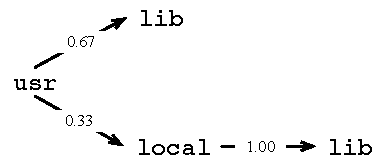
\includegraphics[scale=.7]{figures/host/syscall/probabilistic_tree}
  \caption{Probabilistic tree example.}
  \label{fig:albero}
\end{figure}

\paragraph{Discrete numeric values}
Flags, opening modes, etc. are usually chosen from a limited
set. Therefore we can store all of them along with a discrete
probability. Since in this case two values can only be ``equal'' or
``different'', we set up a binary distance model for clustering.

\begin{definition}[Discrete numeric args. distance]
  Let $x = i_{disc}$, $y = j_{disc}$ be the values of the arguments of
  type \emph{disc} (i.e., discrete numeric argument) of two instances
  $i$ and $j$ of the same system call. The \emph{distance} is defined
  as:

  \begin{displaymath}
    d_{disc}(i,j) := \left\{
      \begin{array}{lll}
        K_{disc} & \mbox{if $x \neq y$}\\
        0 & \mbox{if $x = y$},
    \end{array}
  \right.
\end{displaymath}

where $K_{disc}$ is a configuration parameter.
\end{definition}

Models fusion and incorporation of new elements are straightforward,
as well as the generation of probability for a new input to belong to
the model.

\begin{note}[Configuration parameters]
  According to the experiments described in
  Section~\ref{host:syscall:result-analysis}, the best detection
  accuracy is achieved with the default value of $K_{disc} = 1$. This
  parameter influences the quality of the clustering and thus may need
  to be changed if some particular, pathological false positives need
  to be eliminated in a specific setting.
\end{note}

\paragraph{Execution argument}
We also noticed that execution argument (i.e. the arguments passed to
the \texttt{execve} system call) are difficult to model, but we found the
length to be an extremely effective indicator of similarity of
use. Therefore we set up a binary distance model.

\begin{definition}[Execution arguments distance]
  Let $x = i_{disc}$ and $y = j_{disc}$ be the string values of the
  arguments of type \emph{disc} (i.e., execution argument) of two
  instances $i$ and $j$ of the same system call. The \emph{distance}
  is defined as:

\begin{displaymath}
  d_{arg}(i,j) := \left\{
    \begin{array}{lll}
      K_{arg} & \mbox{if $|x| \neq |y|$}\\
      0 & \mbox{if $|x| = |y|$},
    \end{array}
  \right.
\end{displaymath}

where $K_{arg}$ is a configuration parameter and $|x|$ is the length
of string $x$.
\end{definition}

\begin{note}[Configuration parameters]
  According to the experiments described in
  Section~\ref{host:syscall:result-analysis}, the best detection
  accuracy is achieved with the default value of $K_{arg} = 1$. This
  parameter influences the quality of the clustering and thus may need
  to be changed if some particular, pathological false positives need
  to be eliminated in a specific setting.
\end{note}

In this way, arguments with the same length are clustered
together. For each cluster, we compute the minimum and maximum value
of the length of arguments. Fusion of models and incorporation of new
elements are straightforward. The probability for a new input to
belong to the model is 1 if its length belongs to the interval, and 0
otherwise.

\paragraph{Token arguments}
Many arguments express \texttt{UID}s or \texttt{GID}s, so we developed
an ad-hoc model for \emph{users and groups} identifiers. Our reasoning
is that all these discrete values have three different meanings:
\texttt{UID} 0 is reserved to the super-user, low values usually are
for system special users, while real users have \texttt{UID}s and
\texttt{GID}s above a threshold (usually 1000). So, we divided the
input space in these three groups, and computed the distance for
clustering using the following definition.

\begin{definition}[UID/GID argument distance]
  Let $x = i_{disc}$ and $y = j_{disc}$ be the values of the arguments
  of type \emph{disc} (i.e., \texttt{GID}/\texttt{UID} argument) of
  two instances $i$ and $j$ of the same system call.

\begin{displaymath}
  d_{uid}(i,j) := \left\{
    \begin{array}{lll}
      K_{uid} & \mbox{if $g(x) = g(y)$}\\
      0 & \mbox{if $g(x) \neq g(y)$}
    \end{array}
  \right.,
\end{displaymath}

where $K_{uid}$ is a configuration parameter, the function $g:
\mathbb{N} \mapsto \{groups\}$ and $\{groups\}$ is the set of user
groups.
\end{definition}

Since \texttt{UID}s are limited in number, they are preserved for
testing, without associating a discrete probability to them. Fusion of
models and incorporation of new elements are straightforward. The
probability for a new input to belong to the model is 1 if the UID
belongs to the learned set, and 0 otherwise.

\begin{note}[Configuration parameters]
  According to the experiments described in
  Section~\ref{host:syscall:result-analysis}, the best detection
  accuracy is achieved with the default value of $K_{uid} = 1$. This
  parameter influences the quality of the clustering and thus may need
  to be changed if some particular, pathological false positives need
  to be eliminated in a specific setting.
\end{note}


\begin{table}[p]
  \centering
    \begin{tabular}{rll}
      \toprule
      \textsc{System call} & \multicolumn{2}{c}{\textsc{Model used for the arguments}} \\
      \midrule
      \texttt{open} & \texttt{pathname} & Path\\
      & \texttt{flags} & Discrete Numeric \\
      & \texttt{mode} & Discrete Numeric \\

      \texttt{execve} & \texttt{filename} & Path\\
      & \texttt{argv} & Execution Argument \\ 

      \texttt{setuid} & \texttt{uid} & User/Group\\
      \texttt{setgid} & \texttt{gid} & User/Group\\

      \texttt{setreuid} & \texttt{ruid} & User/Group\\
      \texttt{setregid} & \texttt{euid} & User/Group\\

      \texttt{setresuid, setresgid} & \texttt{ruid} & User/Group\\
      & \texttt{euid} & User/Group\\
      & \texttt{suid} & User/Group\\

      \texttt{symlink, link} & \texttt{oldpath} & Path\\
      \texttt{rename}& \texttt{newpath} & Path\\

      \texttt{mount} & \texttt{source} & Path\\
      & \texttt{target} & Path\\
      & \texttt{flags} & Discrete Numeric\\

      \texttt{umount} & \texttt{target} & Path\\
      & \texttt{flags} & Path\\

      \texttt{exit} & \texttt{status} & Discrete Numeric\\

      \texttt{chown} & \texttt{path} & Path\\
      \texttt{lchown} & \texttt{group} & User/Group\\
      & \texttt{owner} & User/Group\\

      \texttt{chmod, mkdir} & \texttt{path} & Path\\
      \texttt{creat} & \texttt{mode} & Discrete Numeric\\

      \texttt{mknode} & \texttt{pathname} & Path\\
      & \texttt{mode} & Discrete Numeric\\
      & \texttt{dev} & Discrete Numeric\\

      \texttt{unlink, rmdir} & \texttt{pathname} & Path\\
      \bottomrule
    \end{tabular}
    \caption{Association of models to system call arguments in our prototype}
  \label{tab:models-our-proto}
\end{table}

In Table \ref{tab:models-our-proto} we summarize the association of
the models described above with the arguments of each of the system
calls we take into account. This model based clustering is somehow
error prone since we would expect obtained centroids to be more
general and thus somehow to interfere when clustering either new or
old instances. To double check this possible issue we follow a simple
process:

\begin{enumerate}
\item creation of clusters on the training dataset;
\item generation of models from each cluster;
\item use of models to classify the original dataset into clusters,
  and check that inputs are correctly assigned to the same cluster
  they contributed to create.
\end{enumerate}

This is done both for checking the representativeness of the models,
and to double-check that the different distances computed make sense
and separate between different clusters.

\begin{table}[t]
  \centering
    \begin{tabular}{lccc}
      \toprule
      \textsc{Executable} & \textsc{\#elements} & \textsc{\% correct} & \textsc{Conf.}\\
      \midrule
      \texttt{fdformat} & 10 & 100\% & 1\\
      \texttt{eject} & 12 & 100\% & 1\\
      \texttt{ps} & 525 & 100\% & 1\\
      \texttt{telnetd} & 38 & 100\% & 0.954\\
      \texttt{ftpd} & 69 & 97.1\% & 0.675\\
      \texttt{sendmail} & 3211 & 100\% & 0.996\\
      \bottomrule
    \end{tabular}
  \caption{Cluster validation process.}
  \label{tab:cluster-validation}
\end{table}

As Table \ref{tab:cluster-validation} shows, for each program in the
\ac{IDEVAL}\index{IDEVAL} dataset (considering the representative open
system call), the percentage of inputs correctly classified, and a
confidence value, computed as the average ``probability to belong''
computed for each element w.r.t. the cluster it helped to build. The
results are almost perfect, as expected, with a lower value for the
ftpd program, which has a wider variability in file names.

\subsection{Capturing process behavior}
\label{host:syscall:markov}
To take into account the execution context of each system call, we use
a first order Markov chain to represent the program flow. The model
states represent the system calls, or better they represent the
various clusters of each system call, as detected during the
clustering process. For instance, if we detected three clusters in the
\texttt{open} system call, and two in the \texttt{execve} system call, then
the model will be constituted by five states: $\texttt{open}_1$,
$\texttt{open}_2$, $\texttt{open}_3$, $\texttt{execve}_1$,
$\texttt{execve}_2$. Each transition will reflect the probability of
passing from one of these groups to another through the program. As we
already observed in Section~\ref{detection:ad:host}, this approach was
investigated in former literature, but never in conjunction with the
handling of parameters and with a clustering approach.

A time domain process demonstrates a Markov property if the
conditional probability density of the current event, given all
present and past events, depends only on the $K$ most recent
events. $K$ is known as the \emph{order} of the underlying
model. Usually, models of order $K=1$ are considered, because they are
simpler to analyze mathematically. Higher-order models can usually be
approximated with first order models, but approaches for using
high-order Markov models in an efficient manner have also been
proposed, even in the intrusion detection field \citep{high}. A good
estimate of the order can be extracted from data using the criteria
defined in \citep{merhav}; for normal Markov models, a $\chi^2$-test
for first against second order dependency can be used
\citep{chiquadro}, but also an information criterion such as
\ac{BIC}\index{BIC} or \ac{MDL}\index{MDL} can be used.

\subsubsection{Training Phase}
Each execution of the program in the training set is considered as a
sequence of observations. Using the output of the clustering process,
each system call is classified into the correct cluster, by computing the
probability value for each model and choosing the cluster whose models
give out the maximum composite probability along all known models:
$\max(\prod_{i \in \mathrm{M}}{P_i})$. The probabilities of the Markov
model are then straightforward to compute. The final results can be
similar to what is shown in \ref{fig:markov}. On a first sight, this
could resemble a simple Markov chain, however it should be noticed
that each of the state of this Markov model could be mapped into the
set of possible cluster elements associated to it. From this
perspective, it could be seen as a very specific \ac{HMM}\index{HMM}
where states are fully observable through an uniform emission
probability over the associated syscalls\index{syscalls}. By simply turning the
clustering algorithm into one with overlapping clusters we could
obtain a proper \ac{HMM}\index{HMM} description of the user behavior
as it would be if we decide to further merge states together. This is
actually our ongoing work toward full \ac{HMM}\index{HMM} behavior
modeling with the aim, through overlapping syscalls\index{syscalls} clustering, of
improving the performance of the classical Baum-Welch algorithm and
solving the issue of \ac{HMM}\index{HMM} hidden space cardinality
selection~\citep{rabiner}. From our experiments, in the case of the
simple traces like the ones found in the \ac{IDEVAL}\index{IDEVAL}
dataset, the used model suffice so we are working on more complex
scenarios (i.e., new real datasets) to improve in a more grounded way
the proposed algorithm.

This type of model is resistant to the presence of a limited number of
outliers (e.g. abruptly terminated executions, or attacks) in the
training set, because the resulting transition probabilities will drop
near zero. For the same reason, it is also resistant to the presence
of any cluster of anomalous invocations created by the clustering
phase. Therefore, the presence of a minority of attacks in the
training set will not adversely affect the learning phase, which in
turn does not require then an attack-free training set.

The final result can be similar to what is shown in Figure
\ref{fig:markov}. In future extensions, the Markov model could then be
simplified by merging some states together: this would transform it in
a Hidden Markov Model, where the state does not correspond directly to
a system call cluster, but rather to a probability distribution of
possible outcomes. However, the use of \acp{HMM}\index{HMM}
complicates both training and detection phases \citep{rabiner}. From
our experiments, in the case of the simple traces like ones found in
the \ac{IDEVAL}\index{IDEVAL} dataset, this step is unnecessary.

\begin{figure}[t]
  \centering
  \begin{tikzpicture}[node distance=1.8cm,
    every node/.style={font=\footnotesize}]
    \node[state,initial]   (execve0)                         {ex$0$};
    \node[state]           (open24)  [right of=execve0]      {op$24$};
    \node[state]           (open12)  [right of=open24]       {op$12$};
    \node[state]           (open3)   [above right of=open12] {op$3$};
    \node[state]           (open45)  [right of=open12]       {op$45$};
    \node[state]           (rename0) [below right of=open12] {re$0$};
    \node[state]           (setuid0) [right of=rename0]      {se$0$};
    \node[state,accepting] (exit0)   [right of=open3]        {e$0$};

    \path[-stealth] (execve0) edge node [above] {1}    (open24)
                    (open24)  edge node [above] {1}    (open12)
                    (open12)  edge node [above left] {0.33} (open3)
                    (open12)  edge node [above] {0.33} (open45)
                    (open12)  edge node [below left] {0.33} (rename0)
                    (rename0) edge node [above] {1}    (setuid0)
                    (open45)  edge node [above] {1}    (setuid0)
                    (open3)   edge node [above] {0.50} (exit0)
                    (setuid0) edge node [right] {1}    (exit0)
                    (open3)   edge [loop above] node {0.50} ();
  \end{tikzpicture}
  \caption{Example of Markov model.}
  \label{fig:markov}
\end{figure}

\subsubsection{Detection Phase}
For detection, three distinct probabilities can be computed for each executed system call: the probability of the \emph{execution} sequence inside the Markov model up to now, $P_s$; the probability of the \emph{system call} to belong to the best-matching cluster, $P_c$; the \emph{last transition} probability in the Markov model, $P_m$.

The latter two probabilities can be combined into a single ``punctual'' probability of the single system call, $P_p = P_c \cdot P_m$, keeping a separate value for the ``sequence'' probability $P_s$. In order to set appropriate threshold values, we use the training data, compute the lowest probability over all the dataset for that single program (both for the sequence probability and for the punctual probability), and set this (eventually modified by a tolerance value) as the anomaly threshold. The tolerance can be tuned to trade off \ac{DR} for \ac{FPR}.

During detection, each system call is considered in the context of the process. The cluster models are once again used to classify each system call into the correct cluster as explained above: therefore ($P_c = \max(\prod_{i \in \mathrm{M}}{P_i})$). $P_s$ and $P_m$ are computed from the Markov model, and require our system to keep track of the current state for each running process. If either $P_s$ or $P_p = P_c \cdot P_m$ are lower than the anomaly threshold, the process is flagged as malicious.  

\begin{note}[Probability Scaling]
Given an $l$-long sequence of system calls, its sequence probability is $P_{s}(l) = \prod_{i = 0}^{l} P_{p}(i)$ where $P_{p}(i) \in [0,1]$ is the punctual probability of the $i$-th system call in the sequence. Therefore, it is self-evident that $\lim_{l \to +\infty} P_{s}(l) = 0$. Experimentally, we observed that the sequence probability quickly decreases to zero, even for short sequences (on the \ac{IDEVAL}\index{IDEVAL} dataset, we found that $P_{s}(l) \simeq 0$ for $l \geq 25$). This leads to a high number of false positives, since many sequences are assigned probabilities close to zero (thus, always lower than any threshold value).

To overcome this shortcoming, we implemented two probability scaling functions, both based on the geometric mean. As a first attempt, we computed $P_{s}(l) = \sqrt[l]{\prod_{i = 1}^{l} P_{p}(i)}$, but in this case

\begin{displaymath}
  \mathrm{P}\left[\lim_{l \to +\infty} P_{s}(l) = e^{-1}\right] = 1.
\end{displaymath}

\begin{proof}
  Let $\mathrm{G}(P_{p}(1), \ldots, P_{p}(l)) = \sqrt[l]{\prod_{i = 1}^{l} P_{p}(i)}$ the geometric mean of the sample $P_{p}(1), \ldots, P_{p}(l)$. If we assume that the sample is generated by a uniform distribution (i.e., $P_{p}(1), \ldots, P_{p}(l) \sim \mathcal{U}(0,1)$) then $\log P_{p}(i) \sim \mathcal{E}(\beta = 1) \: \forall i = 1, \ldots, l$: this can be proven by observing that the \ac{CDF} \citep{pestman} of $\log X$ (with $X = P_{p} \sim \mathcal{U}(0,1)$) equals the \ac{CDF}\index{CDF} of an exponentially distributed variable with $\beta = 1$.

  The arithmetic mean $\mathrm{A}(\cdot)$ of the sample

  \begin{displaymath}
    -\log(P_{p}(1)), \ldots, -\log(P_{p}(l))
  \end{displaymath}

  converges (in probability) to $\beta = 1$ for $l \to +\infty$, that is:
  \[
  \mathrm{P}\left[\lim_{l \to +\infty} \frac{1}{l}\sum_{i = 1}^{l} -\log P_{p}(i) = -\beta = -1 \right] = 1
  \]

  because of the strong law of large numbers. Being the geometric mean:

  \[
  \mathrm{G}(P_{p}(1), \ldots, P_{p}(l)) = \left(\prod_{i=1}^{l} P_{p}(i)\right)^{\frac{1}{l}} = e^{\frac{1}{l}\sum_{i = 1}^{l} -\log P_{p}(i)}
  \]

  we have

  \[
  \mathrm{P}\left[\lim_{l \to +\infty} \left( e^{\frac{1}{l}\sum_{i = 1}^{l} -\log P_{p}(i)} \right) = e^{-\beta} = e^{-1} \right] = 1
  \]
  \hfill$\qed$
\end{proof}

This is not our desired result, so we modified this formula to introduce a sort of ``forgetting factor'': $P_{s}(l) = \sqrt[2l]{\prod_{i = 1}^{l} P_{p}(i)^{i}}$. In this case, we can prove that $\mathrm{P}\left[\lim_{l \to +\infty} P_{s}(l) = 0\right] = 1$.

\begin{proof}
  The convergence of $P_{s}(l)$ to zero can be proven by observing that:
  \begin{eqnarray*}
    P_{s}(l) & = & \left(\sqrt[l]{\prod_{i = 1}^{l} P_{p}(i)^{i}}\right)^{\frac{1}{2}} = \left(e^{ \frac{1}{l} \sum_{i = 1}^{l} i \cdot \log P_{p}(i) }\right)^{\frac{1}{2}} =\\
    & = & \left(e^{ \frac{1}{l} \sum_{j = 0}^{l} \left( \sum_{i = 1}^{l-j} \log P_{p}(i) \right)}\right)^{\frac{1}{2}} =\\
    & = & \left(e^{ \sum_{j = 0}^{l} \left( \frac{1}{l} \sum_{i = 1}^{l} \log P_{p}(i) - \frac{1}{l} \sum_{i = l-j+1}^{l} \log P_{p}(i) \right)}\right)^{\frac{1}{2}}
  \end{eqnarray*}
  Because of the previous proof, we can write that:
  \[
  \mathrm{P}\left[\lim_{l \to +\infty} \frac{1}{l} \sum_{i = 1}^{l} \log P_{p}(i) = - 1 \right] = 1
  \]
  We can further observe that, being $\log P_{p}(i) < 0$:
  \[
  \forall j, l > 0: \sum_{i = 1}^{l} \log P_{p}(i) < \sum_{i = l-j+1}^{l} \log P_{p}(i)
  \]
  therefore, the exponent is a sum of infinite negative quantities lesser than $0$, leading us to the result that, \emph{in probability}
  \begin{eqnarray*}
    &&\lim_{l \to +\infty} \left(e^{ \sum_{j = 0}^{l} \left( \frac{1}{l} \sum_{i = 1}^{l} \log P_{p}(i) - \frac{1}{l} \sum_{i = l-j+1}^{l} \log P_{p}(i) \right) }\right)^{\frac{1}{2}} =\\
    &&\lim_{x \to -\infty} e^{x} = 0
  \end{eqnarray*}
  \hfill$\qed$
\end{proof}

Even if this second variant once again makes $P_{s}(l) \to 0$ (in probability), our experiments have shown that this effect is much \emph{slower} than in the original formula: $P_{s}(l) \simeq 0$ for $l \geq 300$ (vs. $l \geq 25$ of the previous version), as shown in Figure \ref{fig:normalization}. In fact, this scaling function also leads to much better results in terms of \ac{FPR} (see Section~\ref{host:syscall:result-analysis}).  
\end{note}

\begin{figure}[t]
  \centering
  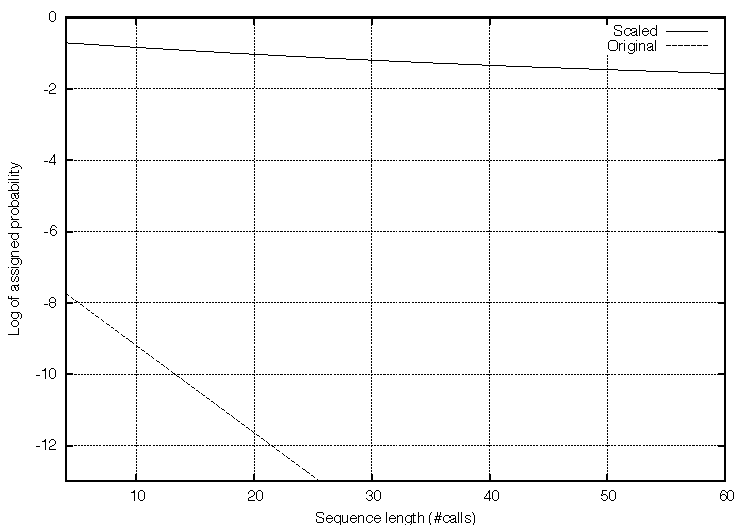
\includegraphics[width=.8\textwidth]{figures/host/syscall/normalization}
  \caption{Measured sequence probability (log) vs. sequence length, comparing the original calculation and the second variant of scaling.}
  \label{fig:normalization}
\end{figure}

Instead of using probabilities --- that are sensitive to the sequence length --- a possible alternative, which we are currently exploring, is the exploitation of distance metrics between Markov models \citep{stolcke93hidden,stolcke:icsi1994:merging,InducingProbabilisticGrammarsMerging} to define robust criteria to compare new and learned sequence models. Basically, the idea is to create and continuously update a Markov model associated to the program instance being monitored, and to check how much such a model differs from the ones the system has learned for the same program. This approach is complementary to the one proposed above, since it requires long sequences to get a proper Markov model. So, the use of both criteria (sequence likelihood in short activations, and model comparison in longer ones) could lead to a reduction of false positives on the sequence model.

\subsection{Prototype implementation}
\label{host:syscall:prot-impl}
We implemented the above described system into a two-stage, highly configurable, modular architecture written in \ac{ANSI}\index{ANSI} C. The high-level structure is depicted in Figure \ref{fig:architetura_hids}: the system is plugged into the Linux \texttt{auditd}. The Cluster Manager is in charge of the clustering phase while the Markov Model Manager implements Markov modeling features. Both the modules are used in both training phase and detection phase, as detailed below.

The Cluster Manager module implements abstract clustering procedures along with abstract representation and storage of generated clusters. The Markov Model Manager is conceptually similar to Cluster Manager: it has a basic Markov chains implementation, along with ancillary modules for model handling and storage.

During training, Cluster Manager is invoked to create the clusters on a given system call trail while Markov Model Manager infers the Markov model according to the clustering. At running time, for each system call, the Cluster Manager is invoked to find the appropriate cluster; the Markov Model Manager is also used to keep track of the current behavior of the monitored process: if significant deviations are found alerts are fired and logged accordingly.

The system can output to both standard output, \texttt{syslog} facilities and \ac{IDMEF}\index{IDMEF} files. Both the clustering phase and the behavioral analysis are multi-threaded and intermediate results of both procedures can be dumped in \ac{XML}\index{XML}.

\begin{figure}[t]
  \hspace*{-.9cm}
  \begin{tikzpicture}[node distance=6.5em,
    every node/.style={text centered,shape=rectangle,draw=black,font=\scriptsize},
    function/.style={font=\scriptsize\itshape,shape=rectangle,draw=black,dashed,thick},
    e/.style={text width=5em,font=\tiny\itshape,draw=none}
    ]

    \node (auditd) {\texttt{auditd}};
    \node [font=\tiny,text width=6em,draw=none,right of=auditd] (syscalls)
    {
      \texttt{execve(args**)}\\
      \texttt{<syscall>(args**)}\\
      \texttt{...}\\
      \texttt{exit()}
    };
    \node (clustering) [text width=3.8em,right of=syscalls] {Cluster Manager};
    \node (mm) [text width=3.8em,right of=clustering] {Markov Model Manager};
    \node (syslogd) at ($ (mm) + (5em,1em) $) {\texttt{syslogd}};
    \node [font=\tiny] (idmef) at ($ (mm) - (-5em,1em) $) {\texttt{<IDMEF />}};

    \node [e] at ($ (auditd) + (0,3em) $) {Kernel\\ Auditing};
    \node [e] at ($ (syscalls) + (0,3em) $) {Syscall \\ Extraction};
    \node [e] at ($ (clustering) + (0,3em) $) {Syscall\\ Classification};
    \node [e] at ($ (mm) + (0,3em) $) {Behavior\\ Modeling};
    \node [e] at ($ (syslogd) + (0,2em) $) {Alerting};

    \draw[-stealth] (auditd) to (syscalls);
    \draw[-stealth] (syscalls) to (clustering);
    \draw[-stealth] (clustering) to (mm);
    \draw[-stealth] (mm) to (syslogd);
    \draw[-stealth] (mm) to (idmef);
  \end{tikzpicture}
  \caption{The high-level structure of our prototype.}
  \label{fig:architetura_hids}
\end{figure}

\subsection{Experimental Results}
\label{host:syscall:result-analysis}
In this section, we both compare the detection accuracy of our
proposal and analyze the performances of the running prototype we
developed. Because of the known issues of \ac{IDEVAL}\index{IDEVAL}
(plus our findings summarized in
Section~\ref{detection:evaluation:darpa}), we also collected fresh
training data and new attacks to further prove that our proposal is
promising in terms of accuracy.

As we detailed in Section~\ref{host:syscall:clust-syst-calls}, our
system can be tuned to avoid overfitting\index{overfitting}; in the current
implementation, such parameters can be specified for \emph{each}
system call, thus in the following we report the bounds of variations
instead of listing \emph{all} the single values: $d_{stop,num} \in
\{1,2,3\}$, $d_{stop,min} = \{6,10,20,60\}$.

\subsubsection{Detection accuracy}
\label{host:syscall:detection-accuracy}
For the reasons outlined above and in
Section~\ref{detection:evaluation:darpa}, as well for the uncertainty
outlined in Section~\ref{host:syscall:crit-libanomaly}, we did not
rely on purely numerical results on \ac{DR} or \ac{FPR}. Instead, we
compared the results obtained by our software with the results of
\SyscallAnomaly in the terms of a set of case studies, comparing them
singularly. What turned out is that our software has two main
advantages over \LibAnomaly:

\begin{itemize}
\item a better contextualization of anomalies, which lets the system
  detect whether a single syscall has been altered, or if a sequence
  of calls became anomalous consequently to a suspicious attack;
\item a strong characterization of subgroups with closer and more
  reliable sub-models.
\end{itemize}

\begin{table}[p]
  \centering
  \begin{tabular}{rl}
    \toprule
    \textsc{HMM State} & \texttt{execve0} (\texttt{START} $\Rightarrow$ \texttt{execve0}) \\
    \cmidrule{2-2}
    filename & \texttt{/usr/bin/fdformat}\\
    argv & \texttt{fdformat$\backslash$0x20$\backslash$0x20$\backslash$0x20$\backslash$0x20[...]} \\
    \cmidrule{2-2}
    $P_c$ & $0.1$ \\
    $P_m$ & $1$ \\
    $P_p$ (thresh.) & $0.1$ ($1$)\\
    \midrule

    \textsc{HMM State} & \texttt{open10} (\texttt{open2} $\Rightarrow$ \texttt{open10}) \\
    \cmidrule{2-2}
    pathname & \texttt{/usr/lib/locale/iso\_8859\_1/[...]}\\
    flags & \texttt{-r-xr-xr-x} \\
    mode & \texttt{33133}\\
    \cmidrule{2-2}
    $P_c$ & $5 \cdot 10^{-4}$ \\
    $P_m$ & $0$ \\
    $P_p$ (thresh.) & $0$ (\emph{undefined})\\
    \midrule

    \textsc{HMM State} & \texttt{open11} (\texttt{open10} $\Rightarrow$ \texttt{open11}) \\
    \cmidrule{2-2}
    pathname & \texttt{/devices/pseudo/vol@0:volctl}\\
    flags & \texttt{crw-rw-rw-} \\
    mode & \texttt{8630}\\
    \cmidrule{2-2}
    $P_c$ & $1$ \\
    $P_m$ & $0$ \\
    $P_p$ (thresh.) & $0$ (\emph{undefined})\\
    \midrule

    \textsc{HMM State} & \texttt{chmod} (\texttt{open11} $\Rightarrow$ \texttt{chmod}) \\
    \cmidrule{2-2}
    pathname & \texttt{/devices/pseudo/vol@0:volctl}\\
    flags & \texttt{crw-rw-rw-} \\
    mode & \texttt{8630}\\
    \cmidrule{2-2}
    $P_c$ & $0.1$\\
    $P_m$ & $0$ \\
    $P_p$ (thresh.) & $0$ (\emph{undefined})\\
    \midrule

    \textsc{HMM State} & \texttt{exit0} (\texttt{chmod} $\Rightarrow$ \texttt{exit0}) \\
    \cmidrule{2-2}
    status & \texttt{0}\\
    \cmidrule{2-2}
    $P_c$ & $1$ \\
    $P_m$ & $0$ \\
    $P_p$ (thresh.) & $0$ (\emph{undefined})\\
    \bottomrule
  \end{tabular}
  \caption{\texttt{fdformat}: attack and consequences}
  \label{tab:fdformat-our-results}
\end{table}

As an example of the first advantage, let us analyze again the program
\texttt{fdformat}, which was already analyzed in
Section~\ref{host:syscall:crit-libanomaly}. As can be seen from Table
\ref{tab:fdformat-our-results}, our system correctly flags
\texttt{execve} as anomalous (due to an excessive length of input). It
can be seen that $P_m$ is 1 (the system call is the one we expected),
but the models of the syscall are not matching, generating a very low
$P_c$. The localization file opening is also flagged as anomalous for
two reasons: scarce affinity with the model (because of the strange
filename), and also erroneous transition between the open subgroups
\texttt{open2} and \texttt{open10}. In the case of such an anomalous
transition, thresholds are shown as ``undefined'' as this transition
has never been observed in training. The attack effect (\texttt{chmod}
and the change of permissions on \texttt{/export/home/elmoc/.cshrc})
and various intervening syscalls\index{syscalls} are also flagged as anomalous because
the transition has never been observed ($P_m = 0$); while reviewing
logs, this also helps us in understanding whether or not the buffer
overflow attack has succeeded. A similar observation can be done on
the execution of \texttt{chmod} on \texttt{/etc/shadow} ensuing an
attack on \texttt{eject}.

In the case of \texttt{ps}, our system flags the \texttt{execve}
system call, as usual, for excessive length of input. File
\texttt{/tmp/foo} is also detected as anomalous argument for
\texttt{open}. In \texttt{LibAnomaly}, this happened just because of
the presence of an underscore, and was easy to bypass. In our case,
\texttt{/tmp/foo} is compared against a sub-cluster of \texttt{open}
which contains only the \texttt{/tmp/ps\_data}, and therefore will
flag as anomalous, with a very high confidence, any other name, even
if structurally similar. A sequence of \texttt{chmod} syscalls\index{syscalls}
executed inside directory \texttt{/home/secret} as a result of the
attacks are also flagged as anomalous program flows.

\begin{table}[t]
  \centering
  \begin{tabular}{cccc}
    \toprule
    & \multicolumn{1}{c}{DR} & \multicolumn{2}{c}{FPR} \\
    \midrule
    \emph{Granularity:} & Sequence & Sequence & Call \\
    \midrule
    Markov model &\multicolumn{3}{c}{\texttt{bsdtar}}\\
    \cmidrule{2-4}
    Y & $100\%$ & $1.6\%$ & $0.1\%$ \\
    N & $88\%$ & $1.6\%$ & $0.1\%$ \\
    \midrule
    &\multicolumn{3}{c}{\texttt{eject}}\\
    \cmidrule{2-4}
    Y & $100\%$ & $0\%$ & $0\%$ \\
    N & $0\%$ & $0\%$ & $0\%$ \\
    \bottomrule
  \end{tabular}
  \caption{\acp{DR}\index{DR} and \acp{FPR}\index{FPR} on two test programs, with (Y) and without (N) Markov models.}
  \label{tab:res-sum}
\end{table}

Limiting the scope to the detection accuracy of our system, we
performed several experiments with both \texttt{eject} and
\texttt{bsdtar}\index{bsdtar}, and we summarize the results in Table
\ref{tab:res-sum}. The prototype has been trained with ten different
execution of \texttt{eject} and more than a hundred executions of
\texttt{bsdtar}\index{bsdtar}. We then audited eight instances of the activity of
\texttt{eject} under attack, while for \texttt{bsdtar}\index{bsdtar} we logged seven
malicious executions. We report \acp{DR}\index{DR} and
\acp{FPR}\index{FPR} with (Y) and without (N) the use of Markov
models, and we compute \acp{FPR}\index{FPR} using cross-validation
through the data set (i.e., by training the algorithm on a subset of
the dataset and subsequently testing the other part of the
dataset). Note that, to better analyze the false positives, we
accounted for both false positive sequences (Seq.) and false positive
system calls (Call).

In both cases, using the complete algorithm yield a 100\% \ac{DR} with
a very low \ac{FPR}. In the case of \texttt{eject}, the exploit is
detected in the very beginning: since a very long argument is passed
to the \texttt{execve}, this triggers the argument model. The
detection of the shellcode\index{shellcode} we injected exploiting the buffer overflow
in \texttt{bsdtar}\index{bsdtar} is identified by the \texttt{open} of the
unexpected (special) file \texttt{/dev/tty}. Note that, the use of
thresholds calculated on the overall Markov model allows us to achieve
a 100\% \ac{DR} in the case of \texttt{eject}; without the Markov
model, the attack wouldn't be detected at all.

\begin{figure}[t]
  \centering
  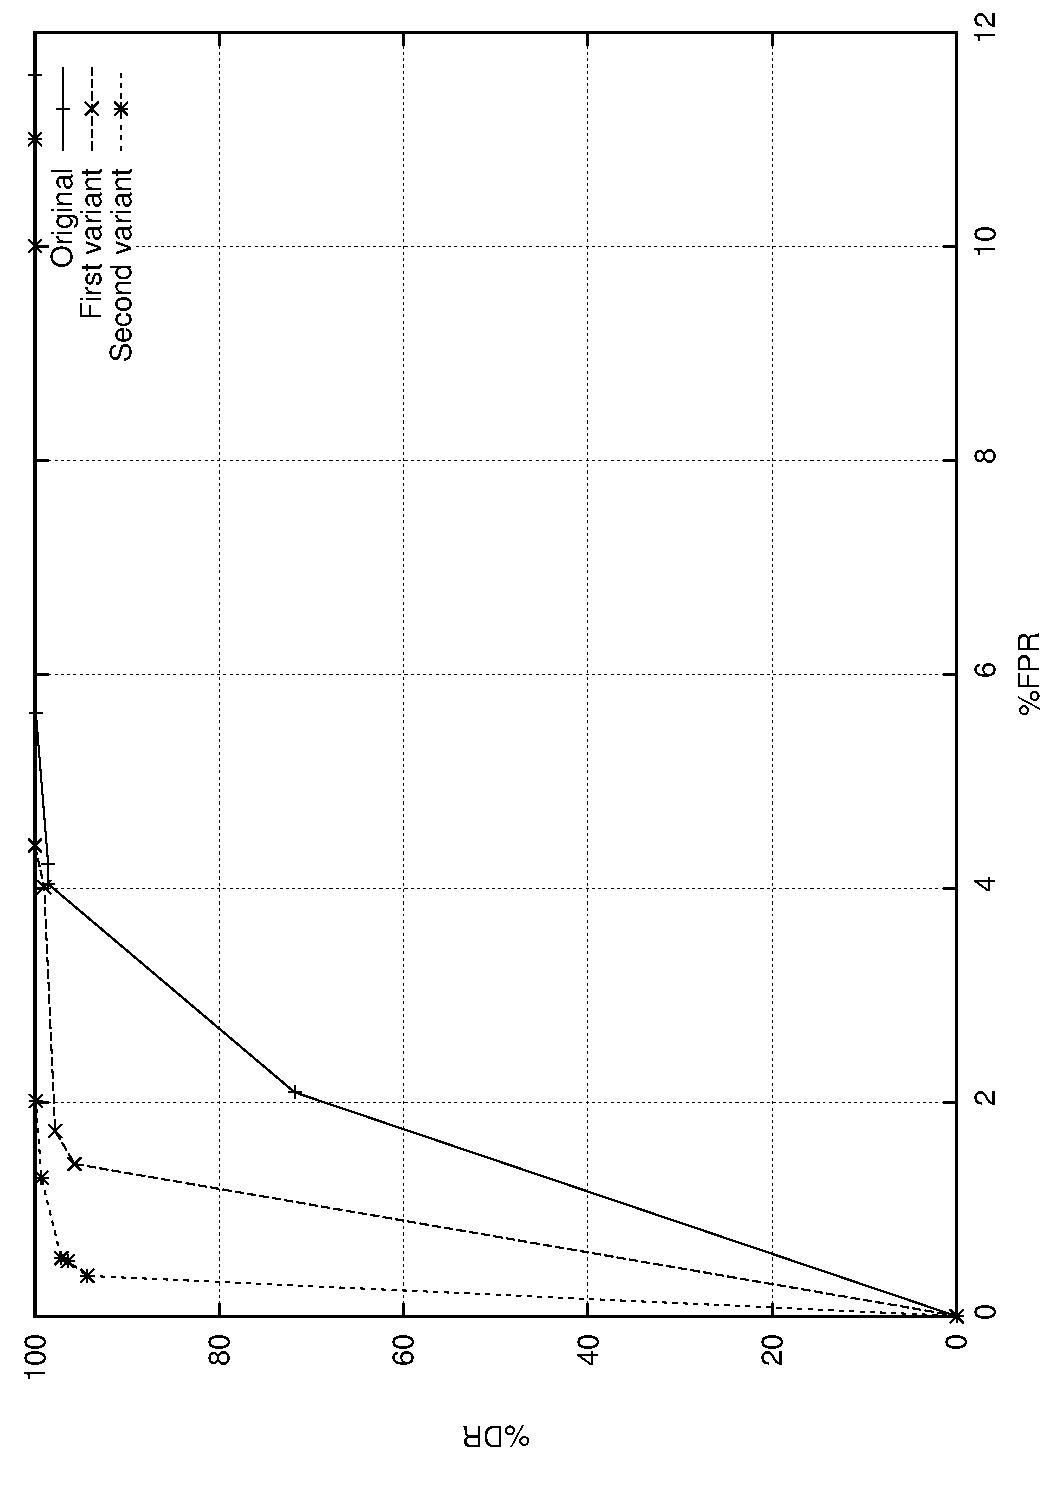
\includegraphics[angle=-90,width=\textwidth]{figures/host/syscall/roc}
  \caption{Comparison of the effect on detection of different probability scaling functions.}
  \label{fig:scaling_comparison}
\end{figure}

It is very difficult to compare our results directly with the other
similar systems we identified in Section~\ref{detection:ad:host}. In
\citep{rulessystemcallarguments} the evaluation is performed on the
\ac{DARPA}\index{DARPA} dataset, but \acp{DR}\index{DR} and
\acp{FPR}\index{FPR} are not given (the number of detections and false
alarms is not normalized), so a direct comparison is
difficult. Moreover, detection is computed using an arbitrary time
window, and false alerts are instead given in ``alerts per day''.  It
is correspondingly difficult to compare against the results in
\citep{venkat_dataflow}, as the evaluation is ran over a dataset which
is not disclosed, using two programs that are very different from the
ones we use, and using a handful of exploits chosen by the
authors. Different scalings of the false positives and
\acp{DR}\index{DR} also make a comparison impossible to draw.

As a side result, we tested the detection accuracy of the two scaling
functions we proposed for computing the sequence probability
$P_{s}$. As shown in Figure \ref{fig:scaling_comparison}, the first
and the second variant both show lower \ac{FPR} w.r.t. to the
original, unscaled version.

\begin{note}[Configuration parameters]
  Although we performed all the experiments with different values of
  $d_{stop,min}$ and $d_{stop,num}$, we report only the best detection
  accuracy, achieved with the default settings: $d_{stop,min} = 10$,
  $d_{stop,num} = 3$.

  These parameters influence the quality of the clustering and thus
  may need to be changed if some particular, pathological false
  positives need to be eliminated in a specific setting. In this case,
  human intervention is required; in particular, it is required to run
  the tool on a small dataset collected on a live system and check the
  clustering for outliers. If clusters containing too many outliers
  exist, then $d_{stop,min}$ may be increased. $d_{stop,num}$ should
  be increased only if outliers cannot be eliminated.
\end{note}

\subsubsection{Performance measurements}
\label{host:syscall:perf-meas}
An \ac{IDS}\index{IDS} should not introduce significant performance overheads in terms of the time required to classify events as malicious (or not). An \ac{IDS}\index{IDS} based on the analysis of system calls has to intercept and process every single syscall invoked on the operating system by userspace\index{userspace} applications; for this reason, the fastest a system call is processed, the best. We profiled the code of our system with \texttt{gprof} and \texttt{valgrind} for \ac{CPU}\index{CPU} and memory requirements. We ran the \ac{IDS}\index{IDS} on data drawn from the \ac{IDEVAL}\index{IDEVAL} 1999 dataset (which is sufficient for performance measurements, as in this case we are only interested in the throughput and not in realistic \acp{DR}\index{DR}).

In Table~\ref{tab:throughput} we reported the measurement of
performance on the five working days of the first week of the dataset
for training, and of the fourth week for testing. The throughput $X$
varies during training between 6120 and 10228 syscalls\index{syscalls}
per second. The clustering phase is the bottleneck in most cases,
while the Markov model construction is generally faster. Due to the
clustering step, the training phase is memory consuming: in the worst
case, we recorded a memory usage of about 700 MB. The performance
observed in the detection phase is of course even more important: in
this case, it varies between 12395 and 22266 syscalls/sec. Considering
that the kernel of a typical machine running services such as
\ac{HTTP}\index{HTTP}/F\ac{TP}\index{TP} on average executes system
calls in the order of thousands per second (e.g., around 2000 system
calls per second for \texttt{wu-ftpd} \citep{mutz06:syscalls}), the
overhead introduced by our \ac{IDS}\index{IDS} is noticeable but does
not severely impact system operations.

\begin{table}[p]
  \centering
  \begin{tabular}{lcccc}
    \toprule
    \multicolumn{5}{c}{\scshape Training throughput}\\
    \midrule
    Ses. & \#Calls & \#Progr. & $t$ (Clust., HMM) [$s$] & $X$ [$call/s$]\\
    \midrule
    1 & 97644 & 111 & 12.056 (7.683, 3.268) & 8099\\ 
    2 & 34931 & 67 & 3.415 (1.692, 1.356) & 10228\\ 
    3 & 41133 & 129 & 6.721 (3.579, 2.677) & 6120\\ 
    4 & 50239 & 152 & 7.198 (3.019, 3.578) & 6979\\ 
    5 & 38291 & 115 & 4.503 (2.219, 1.849) & 8503\\ 
    \midrule
    \multicolumn{3}{l}{Avg. processing time} & $1.2910 \cdot 10^{-4}$ &\\
    \midrule
    \multicolumn{5}{c}{\scshape Detection throughput}\\
    \midrule
    Ses. & \#Calls & \#Progr. & $t$ [$s$] & $X$ [$call/s$]\\
    \midrule
    1 & 109160 & 149 & 6.722 & 16239\\ 
    2 & 160565 & 186 & 12.953 & 12395\\ 
    3 & 103605 & 143 & 4.653 & 22266\\ 
    4 & 115334 & 107 & 5.212 & 22128\\ 
    5 & 112242 & 147 & 5.674 & 19781\\ 
    \midrule
    \multicolumn{3}{l}{Avg. processing time} & $5.6581 \cdot 10^{-5}$ &\\
  \end{tabular}
  
  \caption{Training and detection throughput $X$. On the same dataset,
    the average processing time with \SSAADE disabled is around
    $0.08741084$, thus, in the worst case, \SSAADE introduces a
    $0.1476\%$ overhead (estimated).}
  \label{tab:throughput}
\end{table}

\section{Mixing Deterministic and Stochastic Models}
\label{host:improving}
In this section, we describe an improvement to the syscall-based anomaly detection system described in Section \ref{host:syscall}, which incorporates both the deterministic models of what we called FSA-DF, detailed in \citep{venkat_dataflow} (that we analyzed in detail in Section \ref{detection:ad:host}), and the stochastic models of \ac{SSAADE}. In \citep{2009_frossi_maggi_rizzo_zanero_improving_syscall_models} we propose a number of modifications, described in the following, that significantly improve the performance of both the original approaches. In this section we begin by comparing FSA-DF with \ac{SSAADE} and analyzing their respective performance in terms of detection accuracy. Then, we outline the major shortcomings of the two systems, and propose various changes in the models that can address them. In particular, we kept the deterministic control flow model of FSA-DF and substituted some deterministic dataflow relations with their stochastic equivalent, using the technique described in Section~\ref{host:improving:path-model}. This allowed us to maintain an accurate characterization of the process control flow and, at the same time, to avoid many \ac{FP} due to the deterministic relations among arguments. More precisely, the original learning algorithm of FSA-DF can be schematized as follow:

\begin{pseudo}
  $\forall \mathtt{c} = \langle syscall_{i-1}, syscall_{i} \rangle$
  make_state(c, PC)
  learn_relations(c)
    equal
    elementOf
    subsetOf
    range
    hasExtension
    isWithinDir
    contains
    hasSameDirAs
    hasSameBaseAs
    hasSameExtensionAs
\end{pseudo}

We noticed that simple relations such as \textsf{equal}, \textsf{elementOf}, \textsf{contains} were not suitable for strings. In particular, they raise too many \ac{FP} also in obvious cases like \texttt{``/tmp/php1553''} \emph{vs.} \texttt{``/tmp/php9022''} where the deterministic \texttt{equal} does not hold, but a smoother predicate could easily detect the common prefix, and thus group the two strings in the same class. This problem is clearly extended to the other two relations that are based on string confrontation as well. To mitigate these side-effects, we augmented the learning algorithm as follows:

\begin{pseudo}
  learn_string_domain($\mathtt{syscall}_{i}$)
  $\forall \mathtt{c} = \langle \mathtt{syscall}_{i-1}, \mathtt{syscall}_{i} \rangle$
  make_state(c, PC)
  learn_relations(c)
    save_model
    subsetOf
    range
    hasExtension
    isWithinDir
    hasSameDirAs
    hasSameBaseAs
    hasSameExtensionAs
\end{pseudo}

where the pseudo-function \texttt{learn\_string\_domain} equals to the training of the \ac{SOM} as described in Section~\ref{host:improving:path-model}, and \texttt{save\_model} plays the role the three relations mentioned above. Basically, it stores the \ac{BMU} corresponding to the string arguments of the current system call. The \ac{BMU} is retrieved by querying the \ac{SOM} previously trained. In addition to this, we complemented the resulting system with two new models to cope with \ac{DoS} attacks (see Section~\ref{host:improving:dos-detection-using}) and the presence of outlier in the training dataset (see Section~\ref{host:improving:exec-models}).

We show how targeted modifications of their anomaly models, as opposed to the redesign of the global system, can noticeably improve the overall detection accuracy. Finally, the impact of these modifications are discussed by comparing the performance of the two original implementations with two modified versions complemented with our models.

\subsection{Enhanced Detection Models}
\label{host:improving:improved-models}
The improvements we made focus on \emph{path} and \emph{execution} arguments. A new \emph{string length} model is added exploiting a Gaussian interval as detailed in Section~\ref{host:improving:exec-models}. The new \emph{edge frequency} model described in Section~\ref{host:improving:dos-detection-using} have been added to detect \ac{DoS} attacks. Also, in Section~\ref{host:improving:path-model} we describe how we exploited \ac{SOM} to model the similarity among \emph{path arguments}. The resulting system, Hybrid IDS incorporates the models of FSA-DF and \ac{SSAADE} along with the aforementioned enhancements.

\subsubsection{Arguments Length Using Gaussian Intervals}
\label{host:improving:exec-models}
The model for system call execution arguments implemented in \ac{SSAADE} takes into account the minimum and maximum length of the parameters found during training, and checks whether each string parameter falls into this range (model probability 1) or not (model probability 0). This technique allows to detect common attempts of buffer overflow through the command line, for instance, as well as various other command line exploits. However, such criteria do not model ``how different'' two arguments are to each others; a smoother function is more desirable. Furthermore, the frequency of each argument in the training set is not taken into account at all. Last but not least, the model is not resilient to the presence of attacks in the training set; just one occurrence of a malicious string would increase the length of the maximum interval allowing argument of almost every length.

The improved version of the interval model uses a Gaussian distribution for modeling the argument length $X_{args} = |args|$, estimated from the data in terms of sample mean and sample variance. The anomaly threshold is a percentile $T_{args}$ centered on the mean. Arguments which length is \emph{outside} the stochastic interval are flagged as anomalous. This model is resilient to the presence of outliers in the dataset. The Gaussian distribution has been chosen since is the natural stochastic extension of a range interval for the length. An example is shown in Figure \ref{fig:args_distribution_normal}.

\begin{figure}[t]
  \hspace*{-0.3cm}
  \begin{tabular}{lr}
    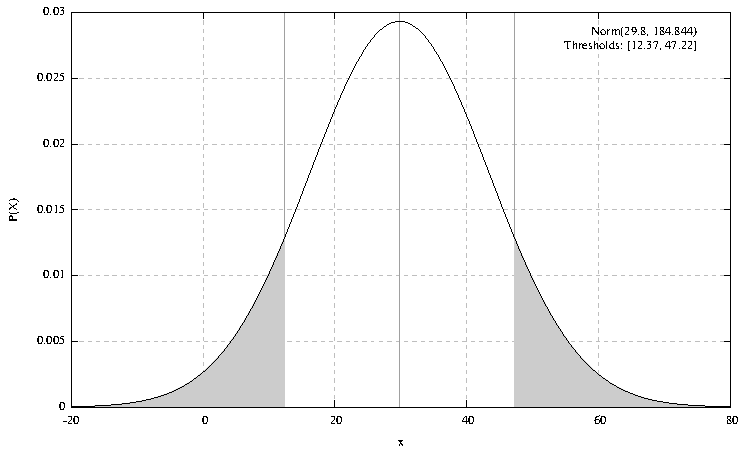
\includegraphics[width=.48\textwidth]{figures/host/improving/args_normal} &
    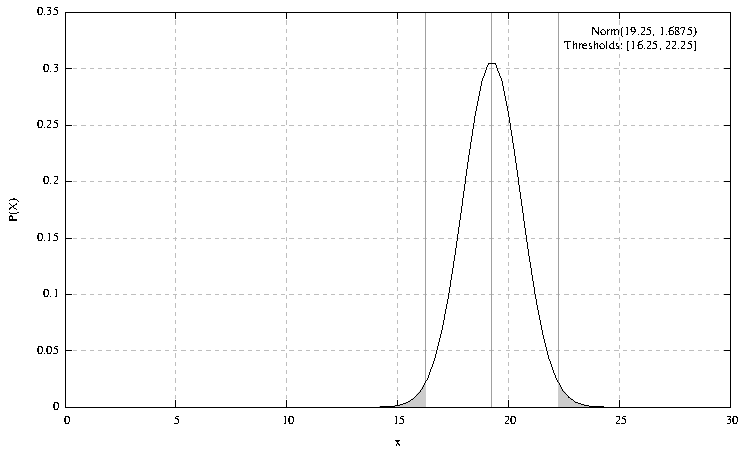
\includegraphics[width=.48\textwidth]{figures/host/improving/args_normal_1}
  \end{tabular}
  \caption[Sample estimated Gaussian intervals for string length.]{Sample estimated Gaussian intervals for string length. Training data of \texttt{sudo} (left) and \texttt{ftp} (right) was used. $\mathcal{N}(29.8, 184.844)$, thresholds [12.37, 47.22] (left) and $\mathcal{N}(19.25, 1.6875)$, thresholds [16.25, 22.25] (right).}
  \label{fig:args_distribution_normal}
\end{figure}

\paragraph{Model Validation} During detection the model self-assesses its precision by calculating the kurtosis measure \citep{joanes1998cms}, defined as $\gamma_{X} = \frac{\mathrm{E}^{4}(X)}{\mathrm{\mathrm{Var}(X)^{2}}}$. Thin tailed distributions with a low peak around the mean exhibit $\gamma_{X} < 0$ while positive values are typical of fat tailed distributions with an acute peak. We used $\hat{\gamma}_{X} = \frac{\mu_{X,4}}{\sigma^{4}_{X}} - 3$ to estimate $\gamma_{X}$. Thus, if $\gamma_{X_{args}} < 0$ means that the sample is spread on a big interval, while positive the values indicates a less ``fuzzy'' set of values. It is indeed straightforward that highly negative values indicates not significant estimations as the interval would include almost all lengths. In this case, the model falls back to a simple interval.

\subsubsection{DoS Detection Using Edge Traversal Frequency}
\label{host:improving:dos-detection-using}
\ac{DoS} attacks which force the process to get stuck in a legal section of the normal control flow could be detected by \ac{SSAADE} as violations of the Markov model, but not by FSA-DF. On the other hand, the statistical models implemented in \ac{SSAADE} are more robust but have higher \acp{FNR}\index{FNR} than the deterministic detection implemented in FSA-DF. However, as already stated in Section~\ref{host:syscall}, the cumulative probability of the traversed edges works well only with execution traces of similar and fixed length, otherwise even the rescaled score decreases to zero, generating false positives on long traces.

\begin{figure}[t]
  \hspace*{-0.3cm}
  \subfloat[][]{
    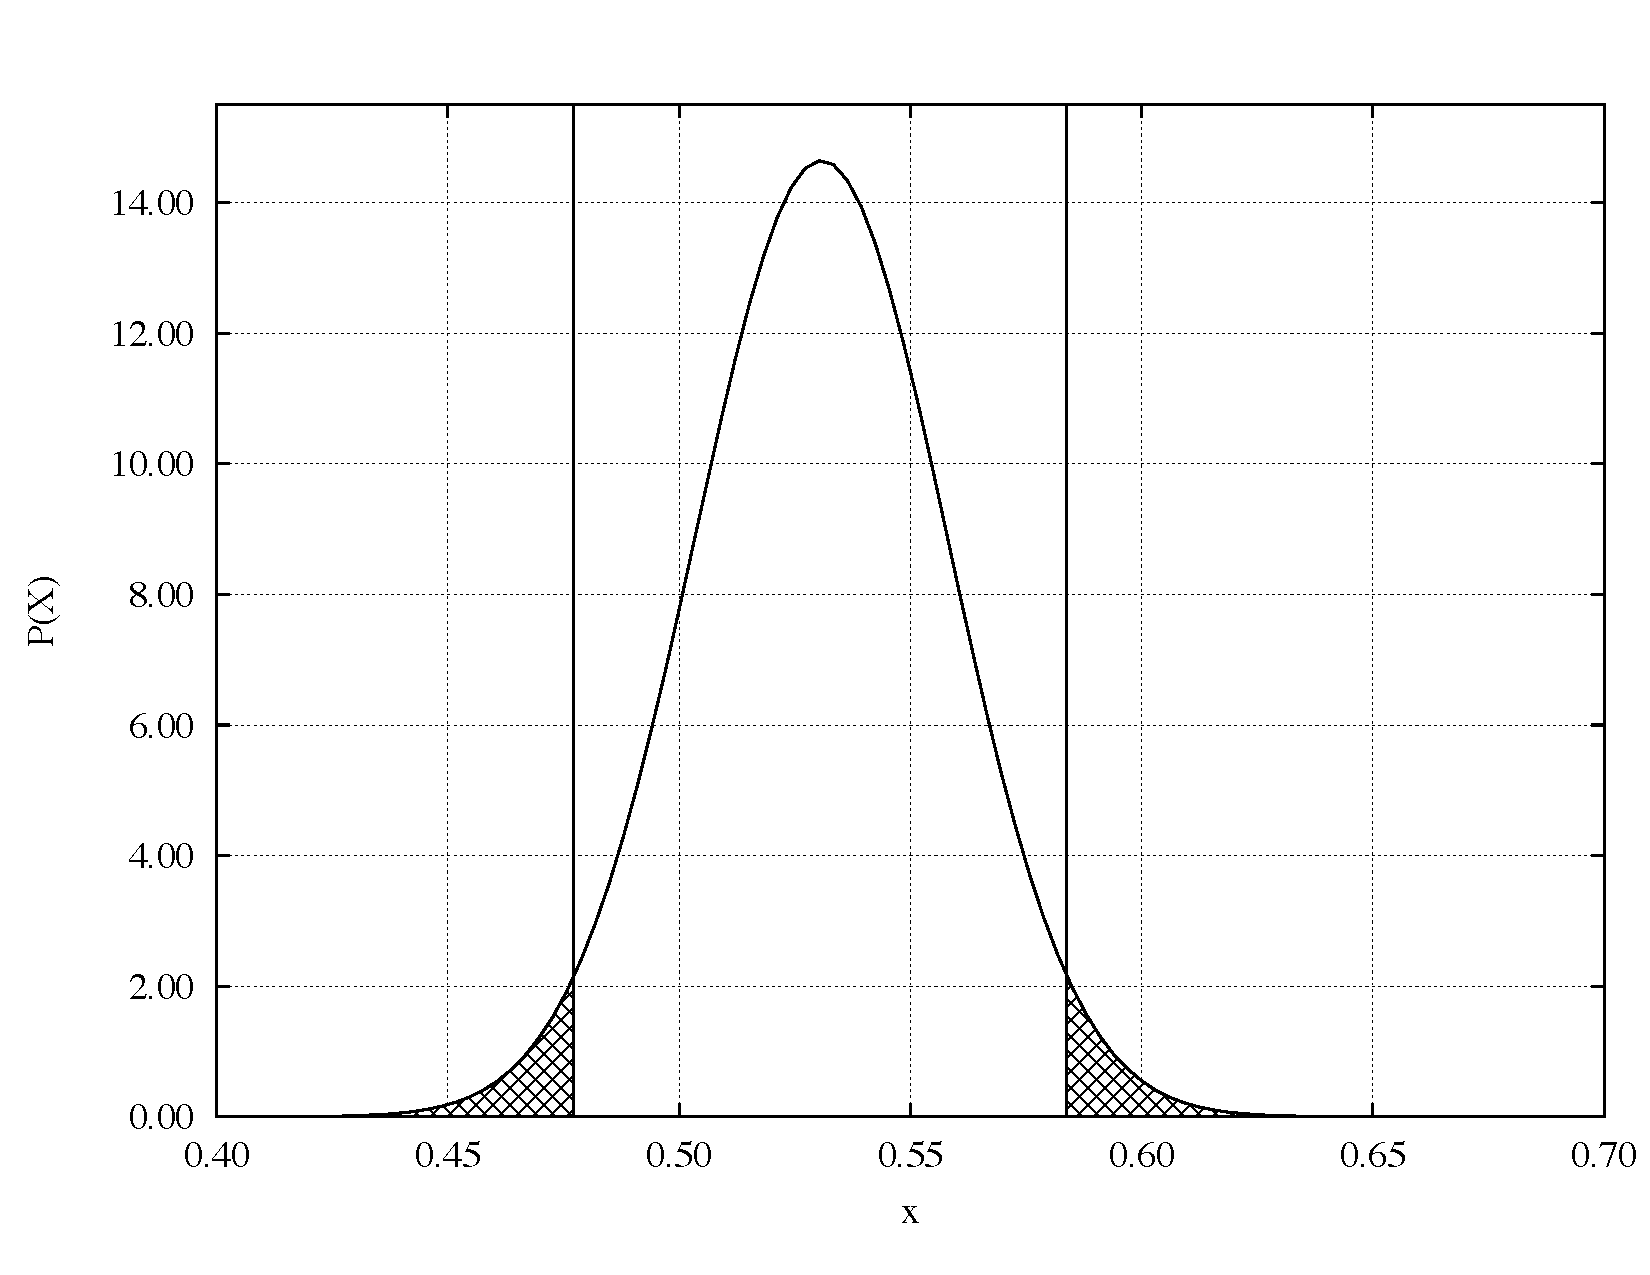
\includegraphics[width=.48\textwidth]{figures/host/improving/beta_left}
  }
  \subfloat[][]{
    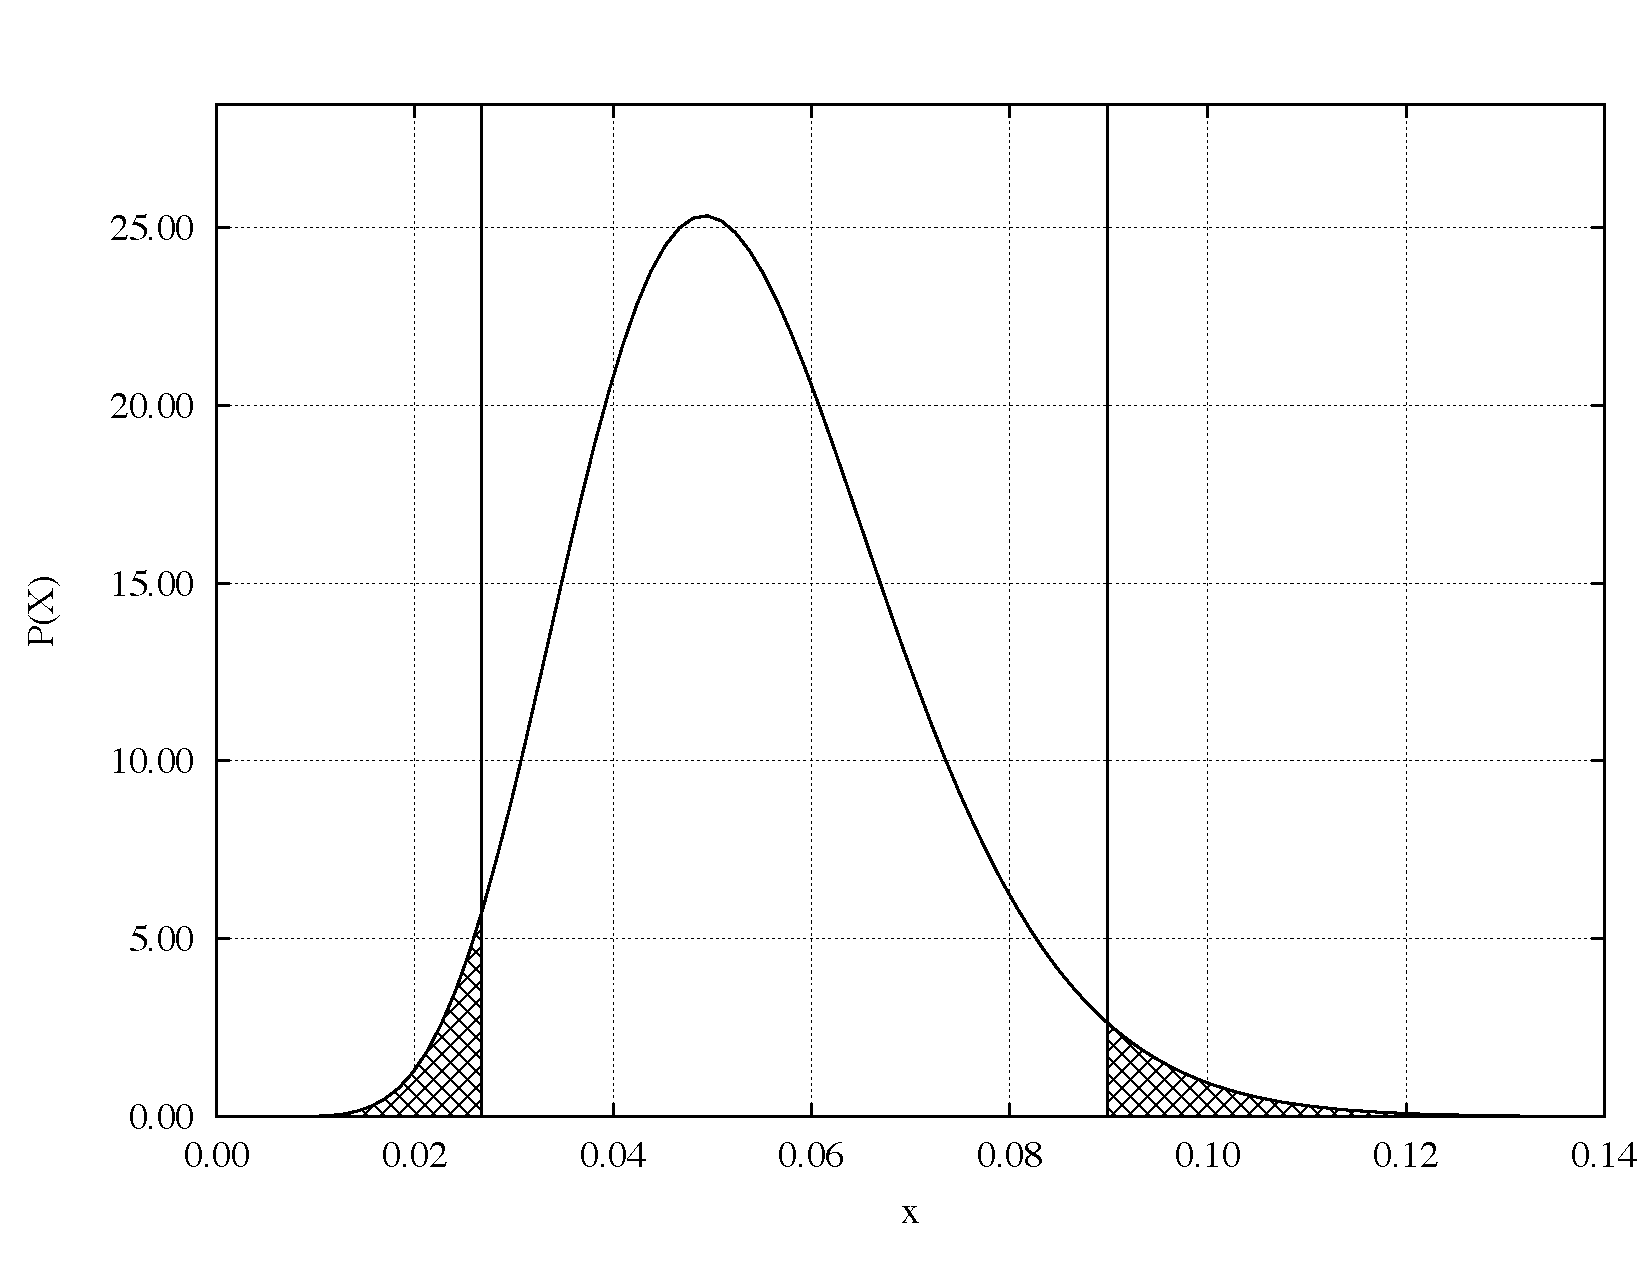
\includegraphics[width=.48\textwidth]{figures/host/improving/beta_right}
  }
  \caption{Two different estimations of the edge frequency distribution. Namely, Beta(178.445, 157.866) with thresholds [0.477199, 0.583649] (left) and Beta(10.3529,181.647) with thresholds [0.0266882, 0.0899057] (right).}
  \label{fig:execve beta}
\end{figure}

To solve these issues a stochastic model of the edge frequency traversal is used. For each trace of the training set, our algorithm counts the number of edge traversals (i.e., Markov model edge or \ac{FSA}\index{FSA} edge). The number is then normalized w.r.t. all the edges obtaining frequencies. Each edge is then associated to the sample $X_{edge} = x_{1}, x_{2}, \dots$. We show that the random samples $X_{edge}$ is well estimated using a Beta distribution. Figure \ref{fig:execve beta} shows sample plots of this model estimated using the \texttt{mt-daapd} training set; the quantiles associated to the thresholds are computed and shown as well. As we did for the Gaussian model, the detection thresholds are defined at configuration time as a percentile $T_{edge}$ centered on the mean (Figure \ref{fig:execve beta}). We chose the Beta for its high flexibility; a Gaussian is unsuitable to model skewed phenomena.

\paragraph{Model Validation} Our implementation is optimized to avoid
overfitting\index{overfitting} and meaningless estimations. A model is
valid only if the training set includes a significant (e.g.,
$|\min_{i}\{x_{i}\} - \max_{i}\{x_{i}\}| \geq \delta x_{min} = 0.04$)
amount ($N_{edge}^{min} = 6$) of paths. Otherwise it construct a
simpler frequency range model. The model exhibits the side effect of
discarding the extreme values found in training and leads to erroneous
decisions. More precisely, if the sample is $X_{edge} = 1, 1, \dots,
0.9, 1$, the right boundary will never be exactly $1$, and therefore
legal values will be discarded. To solve this issue, the quantiles
close to $1$ are approximated to $1$ according to a configuration
parameter $\bar{X}_{cut}$. For instance, if $\bar{X}_{cut} = 3$ the
quantile $F_{X}(\cdot) = 0.99\underline{\bar{9}}$ is approximated to
$1$.

\subsubsection{Path Similarity Using Self Organizing Maps}
\label{host:improving:path-model}
Path argument models are already implemented in \ac{SSAADE} and FSA-DF. Several, general-purpose string comparison techniques have been proposed so far, especially in the field of database systems and data cleansing \citep{elmagarmid2007drd}. We propose a solution based on Symbol-\acp{SOM}\index{SOM} \citep{symbolsom_online} to define an accurate distance metric between paths. Symbol \ac{SOM}\index{SOM} implements a smooth similarity measure otherwise unachievable using common, crisp distance functions among strings (e.g., edit distance).

The technique exploits \acp{SOM}\index{SOM}, which are unsupervised neural algorithms. A \ac{SOM} produces a compressed, multidimensional representation (usually a bi-dimensional \emph{map}) of the input space by preserving the main topological properties. It is initialized randomly, and then adapted via a competitive and cooperative learning process. At each cycle, a new input is compared to the known models, and the \ac{BMU} node is selected. The \ac{BMU} and its neighborhood models are then updated to make them better resemble future inputs.

We use the technique described in \citep{symbolsom_intro} to map \emph{strings} onto \acp{SOM}\index{SOM}. Formally, let

\begin{displaymath}
  S_{t} = [s_{t}(1)\cdots s_{t}(L)]
\end{displaymath}

denote the $t$-th string over the alphabet $\mathcal{A}$ of size $|\mathcal{A}|$. Each symbol $s_{t}(i), i = 1 \ldots L$, is then encoded into a vector $\underline{s}_{t}(i)$ of size $|\mathcal{A}|$ initialized with zeroes except at the $w$-th position which corresponds to the index of the encoded symbol (e.g., $s_{t}(i) = `b'$ would be $\underline{s}_{t}(i) = [0~1~0~0 \cdots 0]^{T}$, $w = 2$). Thus, each string $S_{t}$ is represented with sequence of $L$ vectors like $\underline{s}_{t}(i)$, i.e. a $L \times |\mathcal{A}|$-matrix: $\underline{\underline{S}}_{t}$.

Let $\underline{\underline{S}}_{t}$ and
$\underline{\underline{M}}_{k}$ denote two vector-encoded strings,
where $\underline{\underline{M}}_{k}$ is the model associated with
\ac{SOM}\index{SOM} node $k$. The distance between the two strings is
$D'(S_{t}, M_{k}) = D(\underline{\underline{S}}_{t},
\underline{\underline{M}}_{k})$. $D(\cdot, \cdot)$ is also defined in
the case of $L_{S_{t}} = |S_{t}| \neq |M_{k}| = L_{M_{k}}$ relying on
dynamic time warping techniques to find the best alignment between the
two sequences before computing the distance. Without going into
details, the algorithm \citep{symbolsom_online} aligns the two
sequences $\underline{s}_{t}(i) \in \underline{\underline{S}}_{t},
\underline{m}_{k}(j) \in \underline{\underline{M}}_{k}$ using a
mapping $[\underline{s}_{t}(i), \underline{m}_{k}(j)]$ $\mapsto$
$[\underline{s}_{t}(i(p)), \underline{m}_{k}(j(p))]$ defined through
the warping function $F: [i, j] \mapsto [i(p), j(p)]$:

\begin{displaymath}
  F = [[i(1), j(1)], \dots, [i(p), j(p)], \dots, [i(P), j(P)]].
\end{displaymath}

The distance function $D$ is defined over the warping alignment of size $P$, $D(\underline{\underline{S}}_{t}, \underline{\underline{M}}_{k}) = \sum_{p = 1}^{P} d(i,j)$, which is $P = L_{S_{t}} = L_{M_{k}}$ if the two strings have equal lengths. More precisely:

\begin{displaymath}
  d(i,j) = d(i(p), j(p)) ||\underline{s}_{t}(i(p)) - \underline{m}_{k}(j(p))||.
\end{displaymath}

The distance is defined upon $g_{i,j} = g(i, j)$, the variable which stores the cumulative distance in each trellis point $(i, j) = (i(p), i(p))$. The trellis is first initialized to $0$ in $(0,0)$, to $+\infty$ for both $(0,\cdot)$ and $(\cdot,0)$, otherwise:

\begin{displaymath}
  g(i,j) = \min\left\{
    \begin{array}{l}
      g(i,j-1) + d(i,j)\\
      g(i-1,j-1) + d(i,j)\\
      g(i-1,j) + d(i,j)
    \end{array}\right.
\end{displaymath}

Note that $i \in [1, L_{S_{t}}]$ and $j \in [1, L_{M_{k}}]$ thus the total distance is $D(\underline{\underline{S}}_{t}, \underline{\underline{M}}_{k}) = g(L_{S_{t}}, L_{M_{k}})$. A simple example of distance computation is show in Figure \ref{fig:distance-matrix} ($\mathcal{A}$ is the English alphabet plus extra characters). The overall distance is $D'(S_{t}, M_{k}) = 8.485$. We used a symmetric Gaussian neighborhood function $h$ whose center is located at the \ac{BMU}\index{BMU} $c(t)$. More precisely

\begin{displaymath}
  h(k, c(t), t) = \alpha(t) e^{-\frac{d(c(t),k)}{2\sigma^{2}(t)}}
\end{displaymath}


where $\alpha(t)$ controls the learning rate and $\sigma(t)$ is the actual width of the neighborhood function. The \ac{SOM}\index{SOM} algorithm uses \emph{two} training cycles. During (1) \emph{adaptation} the map is more flexible, while during (2) \emph{tuning} the learning rate $\alpha_{(\cdot)}$ and the width of the neighborhood $\sigma_{(\cdot)}$ are decreased. On each phase such parameters are denoted as $\alpha_{1}, \alpha_{2}, \sigma_{1}, \sigma_{2}$.

\begin{figure}[t]
  \begin{equation*}
     \bordermatrix{
      &&               \mathsf{/}&\mathsf{b}&\mathsf{i}&\mathsf{n}&\mathsf{/}&\mathsf{s}&\mathsf{h} \cr
      &0&+\infty&+\infty&+\infty&+\infty&+\infty&+\infty&+\infty \cr
      \mathsf{/}&+\infty & 0 &  1.414 & 2.828 & 4.242 & 4.242 & 5.656 & 7.071 \cr
      \mathsf{v}&+\infty & 1.414 & 1.414 & 2.828 & 4.242 & 5.656 & 5.656 & 7.071 \cr
      \mathsf{a}&+\infty & 2.828 & 2.828 & 2.828 & 4.242 & 5.656 & 7.071 & 7.071 \cr
      \mathsf{r}&+\infty & 4.242 & 5.656 & 5.656 & 5.656 & 4.242 & 5.656 & 7.071 \cr
      \mathsf{/}&+\infty & 4.242 & 4.242 & 4.242 & 4.242 & 5.656 & 7.071 & 8.485 \cr
      \mathsf{l}&+\infty & 5.656 & 5.656 & 7.071 & 7.071 & 5.656 & 5.656 & 7.071 \cr
      \mathsf{o}&+\infty & 7.071 & 7.071 & 7.071 & 8.485 & 7.071 & 7.071 & 7.071 \cr
      \mathsf{g}&+\infty & 8.485 & 8.485 & 8.485 & 8.485 & 8.485 & 8.485 & \mathbf{8.485}
    }
  \end{equation*}

  \caption{Distance computation example.}
\label{fig:distance-matrix}
\end{figure}

Symbol \acp{SOM}\index{SOM} are ``plugged'' into FSA-DF by associating each transition with the \emph{set} of \acp{BMU}\index{BMU} learned during training. At detection, an alert occurs whenever a path argument falls into neighborhood of a non-existing \ac{BMU}\index{BMU}. Similarly, in the case of \ac{SSAADE}, the neighborhood function is used to decide whether the string is anomalous or not, according to a proper threshold which is the minimum value of the neighborhood function encountered during training, for each node.

\subsection{Experimental Results}
\label{host:improving:accuracy}
In this section we describe our efforts to cope with the lack of reliable testing datasets for intrusion detections. The testing methodology is here detailed along with the experiments we designed. Both detection accuracy and performance overhead are subjects of our tests.

\begin{table}[p]
  \centering\footnotesize
  \begin{tabular*}{\columnwidth}{@{\extracolsep{\fill}}rccccccc}

    \toprule

    & \texttt{sing} & \texttt{mt-daapd} & \texttt{proftpd} & \texttt{sudo} & \multicolumn{1}{c}{\texttt{BitchX}}\\

    \midrule

    SOM & 15 $\times$ 15 & 15 $\times$ 15 & 15 $\times$ 15 & 15 $\times$ 15 & 10 $\times$ 10\\
    Traces & 18 & 18 & 18 & 18 & 14\\
    Syscalls & 5808 & 194879 & 64640 & 52034 & 103148\\
    Paths & 2700 & 2700 & 23632 & 1316 & 14921 \\
    Paths/cycle\% & 2 & 2 & 1 & 8 & 1 \\
    \bottomrule
  \end{tabular*}
  
  \caption{Parameters used to train the \acp{IDS}\index{IDS}. Values includes the number of traces used, the amount of paths encountered and the number of paths per cycle.}
  \label{tab:testing}
\end{table}

In order to evaluate and highlight the impact of each specific model, we performed targeted tests rather than reporting general \acp{DR}\index{DR} and \acp{FPR}\index{FPR} only. Also, we ensured that all possible alerts types are inspected (i.e., true/false positive/negative). In particular, for each \ac{IDS}\index{IDS}, we included one \emph{legal} trace in which file operations are performed on files \emph{never} seen during training but with a similar name (e.g., training on \texttt{/tmp/log}, testing on \texttt{/tmp/log2}); secondly, we inserted a trace which mimics an attack.

\subsubsection{Comparison of Detection Accuracy}
\label{host:improving:test_hybrid}
The detection accuracy of Hybrid IDS (H), FSA-DF (F) and \ac{SSAADE} (S) is here analyzed and compared. Both training parameters and detection results are summarized in Table \ref{tab:testing}. The parameters used to train the \ac{SOM}\index{SOM} are fixed except for $\sigma_{1}(t)$: $\alpha_{1}(t) = 0.5\div0.01$, $\sigma_{2}(t) = 3$ and $\alpha_{2}(t) = 0.1\div0.01$. Percentiles for both $X_{args}$ and $X_{edge}$ are detailed. The ``paths/cycle\%'' (paths per cycle) row indicates the amount of paths arguments used for training the \ac{SOM}\index{SOM}. The settings for clustering stage of \ac{SSAADE} are constant: minimum number of clusters ($3$, or $2$ in the case of the \texttt{open}); maximum merging distance ($6$, or $10$ in the case of the \texttt{open}); the ``null'' and the ``don't care'' probability values are fixed at $0.1$ and $10$, respectively, while $10$ is the maximum number of leaf clusters. In order to give a better understanding of how each prototype works, we analyzed by hand the detection results on each target application.

\begin{table}[p]
  \centering\footnotesize
  \begin{tabular*}{\columnwidth}{@{\extracolsep{\fill}}rccccccc}

    \toprule

       & \texttt{sing} & \texttt{mt-daapd} & \texttt{profdtpd} & \texttt{sudo} & \multicolumn{1}{c}{\texttt{BitchX}}\\

    \midrule

    Traces & 22 & 18 & 21 & 22 & 15\\
    Syscalls & 1528 & 9832 & 18114 & 3157 & 107784\\
    \ac{SSAADE} & 10.0\% & 0\% & 0\% & 10.0\% & 0.0\%\\
    FSA-DS & 5.0\% & 16.7\% & 28\% & 15.0\% & 0.0\%\\
    Hybrid IDS & 0.0\% & 0\% & 0\% & 10.0\% & 0.0\%\\

    \bottomrule
  \end{tabular*}
  
  \caption{Comparison of the \ac{FPR} of \ac{SSAADE} vs. FSA-DF vs. Hybrid IDS. Values include the number of traces used. Accurate description of the impact of each \emph{individual} model is in Section~\ref{host:improving:test_hybrid}}
  \label{tab:testing2}
\end{table}

\begin{description}
  \item [\texttt{sing}:] Hybrid IDS is not tricked by the false positive mimic trace inserted. The Symbol SOM model recognizes the similarity of \texttt{/tmp/log3} with the other paths inserted in the training. Instead, both FSA-DF and \ac{SSAADE} raise false alarms; the former has never seen the path during training while the latter recognizes the string in the tree path model but an alarm is raised because of threshold violation. \ac{SSAADE} recognizes the attack containing the longer subsequent invocations of \texttt{mmap2}; FSA-DF also raises a violation in the file name because it has never been trained against \texttt{/etc/passwd} nor \texttt{/etc/shadow}; and Hybrid IDS is triggered because the paths are placed in a different \ac{SOM}\index{SOM} region w.r.t. the training.
  \item[\texttt{mt-daapd}:] The legit traces violate the binary and unary relations causing several false alarms on FSA-DF. On the other hand, the smoother path similarity model allows Hybrid IDS and \ac{SSAADE} to pass the test with no false positives. The changes in the control flow caused by the attacks are recognized by all the \acp{IDS}\index{IDS}. In particular, the DoS attack (special-crafted request sent fifty times) triggers an anomaly in the edge frequency model.
  \item[\texttt{proftpd}:] The legit trace is correctly handled by all the \acp{IDS}\index{IDS} as well as the anomalous root shell that causes unexpected calls (\verb#setuid#, \verb#setgid# and \verb#execve#) to be invoked. However, FSA-DF flags more than 1000 benign system calls as anomalous because of temporary files path not present in the training.
\item [\texttt{sudo}:] Legit traces are correctly recognized by all the engines and attacks are detected without errors. \ac{SSAADE} fires an alert because of a missing edge in the Markov model (i.e., the unexpected execution of \texttt{chown root:root script} and \texttt{chmod +s script}). Also, the absence of the \texttt{script} string in the training triggers a unary relation violation in FSA-DF and a \ac{SOM}\index{SOM} violation in Hybrid IDS. The traces which mimic the attack are erroneously flagged as anomalous, because the system call sequences are \emph{strictly} similar to the attack.
\item [\texttt{BitchX}:] The exploit is easily detected by all the \acp{IDS}\index{IDS} as a control flow violation through extra \texttt{execve} system calls are invoked to execute injected commands. Furthermore, the Hybrid IDS anomaly engine is triggered by three edge frequency violations due to paths passed to the \ac{FSA}\index{FSA} when the attack is performed which are different w.r.t. the expected ones.
\end{description}

\subsubsection{Specific Comparison of SOM-\ac{SSAADE} and \ac{SSAADE}}
\label{host:improving:test_som}
We also specifically tested how the introduction of a Symbol \ac{SOM}\index{SOM} improves over the original probabilistic tree used for modeling the path arguments in \ac{SSAADE}. Training parameters are reported in Table \ref{tab:testing-som} while results are summarized in Table \ref{tab:testing2-som}, the \ac{FPR} decreases in the second test. However, the first test exhibits a lower \ac{FNR} as detailed in the following.

\begin{table}[p]
  \centering
  \begin{tabular*}{\columnwidth}{@{\extracolsep{\fill}}rcc}

    \toprule

    & \texttt{mcweject} & \texttt{bsdtar} \\

    \midrule

    SOM & 15 $\times$ 15 & 15 $\times$ 15\\
    Traces & 10 & 240 \\
    Syscalls & 84 & 12983\\
    Paths & 48 & 3477 \\
    Paths/cycle\% & 50 & 2 \\
    \bottomrule
  \end{tabular*}
  
  \caption{Parameters used to train the \acp{IDS}\index{IDS}. Values includes the number of traces used, the amount of paths encountered and the number of paths per cycle.}
  \label{tab:testing-som}
\end{table}

The \texttt{mcweject}\index{mcweject} utility is affected by a stack overflow CVE-2007-1719 caused by improper bounds checking. Root privileges can be gained if \texttt{mcweject}\index{mcweject} is \texttt{setuid}. Launching the exploit is as easy as \texttt{eject -t illegal\_payload}, but we performed it through the userland\index{userland} execution technique we describe in Section~\ref{host:forensics:antifor} to make it more stealthy avoiding the \texttt{execve} that obviously triggers an alert in the \ac{SSAADE} for a missing edge in the Markov chain. Instead, we are interested in comparing the string models only. SOM-\ac{SSAADE} detects it with no issues because of the use of different ``types'' of paths in the \texttt{open}s.

An erroneous computation of a buffer length is exploited to execute code via a specially crafted PAX archives passed to \texttt{bsdtar}\index{bsdtar} (CVE-2007-3641). A heap overflow allows to overwrite a structure pointer containing itself another pointer to a function called right after the overflow. The custom exploit \citep{zanero_self} basically redirects that pointer to the injected shellcode\index{shellcode}. Both the original string model and the Symbol \ac{SOM}\index{SOM} models detect the attack when an unexpected special file (i.e., \texttt{/dev/tty}) is opened. However, the original model raises many false positives when significantly different paths are encountered. This situation is instead handled with no false positives by the smooth Symbol \ac{SOM}\index{SOM} model.

\begin{table}[p]
  \centering
  \begin{tabular*}{\columnwidth}{@{\extracolsep{\fill}}rcc}

    \toprule

    & \texttt{mcweject} & \texttt{bsdtar} \\

    \midrule

    Traces & 12 & 2 \\
    Syscalls & 75 & 102\\
    \ac{SSAADE} & 0.0\% & 8.7\%\\
    SOM-\ac{SSAADE} & 0.0\% & 0.0\%\\
    \bottomrule
  \end{tabular*}
  
  \caption{Comparison of the \ac{FPR} of \ac{SSAADE} vs. SOM-\ac{SSAADE}. Values include the number of traces used.}
  \label{tab:testing2-som}
\end{table}

Since this dataset has been originally prepared for \citep{zanero_self,10.1109/TDSC.2008.69}, details on its generation are described in Section~\ref{host:experimental-setup}.

\subsubsection{Performance Evaluation and Complexity Discussion}
\label{host:improving:test_performance}
We performed both empirical measurements and theoretical analysis of the performance of the various proposed prototypes. Detection speed results are summarized in Table \ref{tab:performance_measurements}. The datasets for detection accuracy were reused: we selected the five test applications on which the \acp{IDS}\index{IDS} performed worst. Hybrid IDS is slow because the \ac{BMU}\index{BMU} algorithm for the symbol \ac{SOM}\index{SOM} is invoked for each system call with a path argument (\texttt{open}s are quite frequent), slowing down the detection phase. Also, we recall that the current prototype relies on a system call interceptor based on \texttt{ptrace} which \emph{introduces high runtime overheads}, as shown in \citep{venkat_dataflow}. To obtain better performance, an in-kernel interceptor could be used. The theoretical performance of each engine can be estimated by analyzing the bottleneck algorithm.

\begin{table}[t]
  \centering\footnotesize

  \begin{tabular*}{\columnwidth}{@{\extracolsep{\fill}}rcccccc}
    \toprule

     & \texttt{sing} & \texttt{sudo} & \texttt{BitchX} & \texttt{mcweject} & \texttt{bsdtar} &\\

    \cmidrule{1-6}

    System calls & 3470 & 15308 & 12319 & 97 & 705 & Speed\\
    
    \midrule

    \ac{SSAADE} & 0.4 & 0.8 & 1.9 & 0.1 & 0.1 & 8463 \\
    FSA-DF & 1.3  & 1.5 & 1.2 & - & - & 7713 \\
    Hybrid IDS & 29 & 5.8 & 27.7 & - & - & 1067 \\
    SOM-\ac{SSAADE} & - & - & - & 8.8 & 19 & 25 \\

    \bottomrule
  \end{tabular*}
  \caption{Detection performance measured in ``seconds per system call''. The average speed is measured in system calls per second (last column).}
  \label{tab:performance_measurements}
\end{table}

\subsubsection{Complexity of FSA-DF}
During training, the bottleneck is the binary relation learning algorithm. $T_{F}^{train} = O(S \cdot M + N)$, where $M$ is the total number of system calls, $S = |Q|$ is the number of states of the automaton, and $N$ is the sum of the length of all the string arguments in the training set. At detection $T_{FSA-DF}^{det} = O(M + N)$.

Assuming that each system call has $O(1)$ arguments, the training algorithm is invoked $O(M)$ times. The time complexity of each $i$-th iteration is $Y_{i} + |X_{i}|$, where $Y_{i}$ is the time required to compute all the unary and binary relations and $|X_{i}|$ indicates the time required to process the $i-th$ system call $X$. Thus, the overall complexity is bounded by $\sum^{M}_{i=1} Y + |X_{i}| = M \cdot Y + \sum^{M}_{i=1} |X_{i}|$. The second factor $\sum^{M}_{i=1} |X_{i}|$ can be simplified to $N$ because strings are represented as a tree; it can be shown \citep{venkat_dataflow} that the total time required to keep the longest common prefix information is bounded by the total length of all input strings. Furthermore, $Y$ is bounded by the number of unique arguments, which in turn is bounded by $S$; thus, $T^{train}_{F} = O(S \cdot M + N)$. This also prove the time complexity of the detection algorithm which, at each state and for each input, requires unary and binary checks to be performed; thus, its cost is bounded by $M + N$.\hfill $\qed$\\

\subsubsection{Complexity of Hybrid IDS}
In the training phase, the bottleneck is the Symbol \ac{SOM}\index{SOM} creation time: $T^{train}_{H} = O(C \cdot D \cdot (L^{2} + L))$, where $C$ is the number of learning cycles, $D$ is the number of nodes, and $L$ is the maximum length of an input string. At detection time $T^{det}_{H} = O(M \cdot D \cdot L^{2})$.

$T^{train}_{H}$ depends on both the number of training cycles, the BMU algorithm and node updating. The input is randomized at each training session and a constant amount of paths is used, thus the input size is $O(1)$. The \ac{BMU}\index{BMU} algorithm depends on both the \ac{SOM}\index{SOM} size and the distance computation, bounded by $L_{input} \cdot L_{node}=L^{2}$, where $L_{input}$ and $L_{node}$ are the \emph{lengths} of the input string and the node string, respectively. More precisely, the distance between strings is performed by comparing all the vectors representing, respectively, each character of the input string and each character of the node string. The char-by-char comparison is performed in $O(1)$ because the size of each character vector is fixed. Thus, the distance computation is bounded by $L^{2} \simeq L_{input} \cdot L_{node}$. The node updating algorithm depends on both the number of nodes $D$, the length of the node string $L_{node}$ and the training cycles $C$, hence each cycle requires $O(D \cdot (L^{2} + L))$, where $L$ is the length of the longest string. The creation of the \ac{FSA}\index{FSA} is similar to the FSA-DF training, except for the computation of the relations between strings which time is no longer $O(N)$ but it is bounded by $M \cdot D \cdot L^{2}$ (i.e., the time required to find the Best Matching Unit for one string). Thus, according to \emph{Proof 1}, this phase requires $O(S \cdot M + M \cdot D \cdot L^{2}) < O(C \cdot D \cdot (L^{2} + L))$. The detection time $T_{H}^{det}$ is bounded by the \ac{BMU}\index{BMU} algorithm, that is $O(M \cdot D \cdot L^{2})$.\hfill$\qed$\\

The clustering phase of \ac{SSAADE} is $O(N^{2})$ while with SOM-\ac{SSAADE} it grows to $O(N^{2}L^{2})$.

In the worst case, the clustering algorithm used in \citep{10.1109/TDSC.2008.69} is known to be $O(N^{2})$, where $N$ is the number of system calls: the distance function is $O(1)$ and the distance matrix is searched for the two closest clusters. In the case of SOM-\ac{SSAADE}, the distance function is instead $O(L^{2})$ as it requires one run of the \ac{BMU}\index{BMU} algorithm.\hfill$\qed$

\section{Forensics Use of Anomaly Detection Techniques}
\label{host:forensics}
Anti-forensics is the practice of circumventing classical forensics
analysis procedures, making them unreliable or impossible. In this
section we describe how machine learning algorithms and anomaly
detection techniques can be exploited to cope with a wide class of
definitive anti-forensics techniques. In \citep{zanero_self} we tested
\ac{SSAADE}, described in Section~\ref{host:syscall} including the
improvements detailed in Section~\ref{host:improving}, on a dataset we
created through the implementation of an innovative technique of
anti-forensics, and we show that our approach yields promising results
in terms of detection.

Computer forensics is usually defined as the process of applying
scientific, repeatable analysis processes to data and computer
systems, with the objective of producing evidence that can be used in
an investigation or in a court of law. More in general, it is the set
of techniques that can be applied to understand if, and how, a system
has been used or abused to commit mischief \citep{mohay}. The
increasing use of forensic techniques has led to the development of
anti-forensic techniques that can make this process difficult, or
impossible \citep{garfinkel,berghel,ryan}.

Anti\hyp{}forensics techniques can be divided into at least two
groups, depending on their target. If the \emph{identification} phase
is targeted, we have \emph{transient} anti-forensics techniques, which
make the acquired evidence difficult to analyze with a specific tool
or procedure, but not impossible to analyze in general. If instead the
\emph{acquisition} phase is targeted, we have the more effective class
of \emph{definitive} anti-forensics techniques, which effectively deny
once and forever any access to the evidence. In this case, the
evidence may be destroyed by the attacker, or may simply not exist on
the media. This is the case of in-memory injection techniques that are
described in the following.

In particular, we propose the use of machine learning algorithms and
anomaly detectors to circumvent such techniques. Note that, referring
once again to the aforementioned definition of computer forensics
in~\citep{mohay}, we focused only on detecting \emph{if} a system has
been compromised. In fact, if definitive anti-forensics techniques can
make it impossible to detect \emph{how} the system has been
exploited. We illustrate a prototype of anomaly detector which
analyzes the sequence and the arguments of system calls to detect
intrusions. We also use this prototype to detect in-memory injections
of executable code, and in-memory execution of binaries (the so-called
``userland\index{userland} exec'' technique, which we re-implement in a reliable
way). This creates a usable audit trail, without needing to resort to
complex memory dump and analysis operations
\citep{burdach,ring2004vmc}.

\subsection{Problem statement}
\label{host:forensics:antifor}
Anti-forensics is defined by symmetry on the traditional definition of computer forensics: it is the set of techniques that an attacker may employ to make it difficult, or impossible, to apply scientific analysis processes to the computer systems he penetrates, in order to gather evidence \citep{garfinkel,berghel,ryan}. The final objective of anti-forensics is to reduce the quantity and spoil the quality \citep{grugq} of the evidence that can be retrieved by an investigation and subsequently used in a court of law.

Following the widely accepted partition of forensics \citep{pollitt} in \emph{acquisition}, \emph{identification}, \emph{evaluation}, and \emph{presentation}, the only two phases where technology can be critically sabotaged are both acquisition and identification. Therefore, we can define anti-forensics as follows.

\begin{definition}[Anti-forensics]
  \emph{Anti-forensics} is a combination of all the methods that make acquisition, preservation and analysis of computer-generated and computer-stored data difficult, unreliable or meaningless for law enforcement and investigation purposes.
\end{definition}

Even if more complex taxonomies have been proposed \citep{ryan}, we can use the traditional partition of the forensic process to distinguish among two types of anti-forensics:

\begin{description}
\item [Transient anti-forensics] when the \emph{identification} phase is targeted, making the acquired evidence difficult to analyze with a specific tool or procedure, but not impossible to analyze in general.
\item [Definitive anti-forensics] when the \emph{acquisition} phase is targeted, ruining the evidence or making it impossible to acquire.
\end{description}

Examples of transient anti-forensics techniques are the fuzzing and abuse of file-systems in order to create malfunctions or to exploit vulnerabilities of the tools used by the analyst, or the use of log analysis tools vulnerabilities to hide or modify certain information \citep{foster,grugq}. In other cases, entire file-systems have been hidden inside the metadata of other file-systems \citep{grugq}, but techniques have been developed to cope with such attempts \citep{det-hidd}. Other examples are the use of steganography \citep{johnson1998ess}, or the modification of file metadata in order to make filetype not discoverable. In these cases the evidence is not completely unrecoverable, but it may escape any quick or superficial examination of the media: a common problem today, where investigators are overwhelmed with cases and usually under-trained, and therefore overly reliant on tools.

Definitive anti-forensics, on the other hand, effectively denies access to the evidence. The attackers may encrypt it, or securely delete it from file-systems (this process is sometimes called ``counter-forensics'') with varying degrees of success \citep{counterfor,garfinkel2003rdp}. Access times may be rearranged to hide the time correlation that is usually exploited by analysts to reconstruct the events timeline. The final anti-forensics methodology is not to leave a trail: for instance, modern attack tools (commercial or open source) such as \textsf{Metasploit} \citep{mafia}, \textsf{Mosdef} or \textsf{Core IMPACT} \citep{coreimpact} focus on pivoting and in-memory injection of code: in this case, nothing or almost nothing is written on disk, and therefore information on the attack will be lost as soon as it is powered down, which is usually standard operating procedure on compromised machines. These techniques are also known as ``disk-avoiding'' procedures.

Memory dump and analysis operations have been advocated in response to this, and tools are being built to cope with the complex task of the reliable acquisition \citep{burdach,body} and analysis \citep{burdach,ring2004vmc,fatkit} of a modern system's memory. However, even in the case that the memory can be acquired and examined, if the process injected and launched has already terminated, once more, no trace will be found of the attack: these techniques are much more useful against in-memory resident backdoors\index{backdoors} and rootkits, which by definition are persistent.

\subsection{Experimental Results}
\label{host:forensics:setup}

\begin{figure}[t]
 \centering
 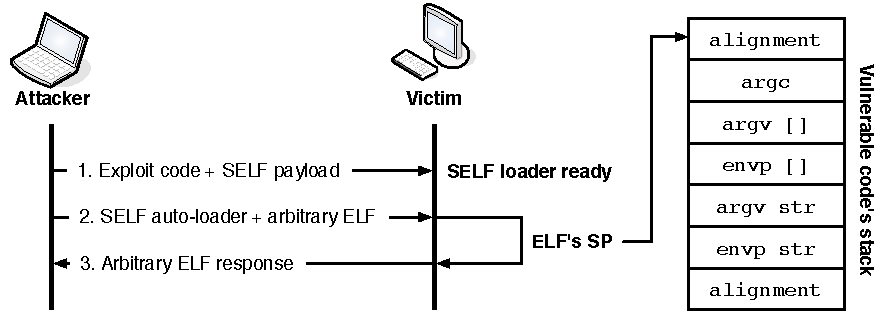
\includegraphics[width=\textwidth]{figures/host/forensics/self_new}
 \caption{An illustration of the in-memory execution technique.}
 \label{fig:self}
\end{figure}

Even in this evaluation, we used the dataset described in
Section~\ref{host:experimental-setup}. However, a slight modification
of the generation mechanism was needed. More precisely, in the tests
conducted we used a modified version of SELF \citep{SELF-TOOL}, which
we improved in order to reliably run under \textsf{FreeBSD}\index{FreeBSD} 6.2 and
ported to a form which could be executed through code injection (i.e.,
to shellcode\index{shellcode} format). SELF implements a technique known as
\emph{userland exec}: it modifies any statically linked
\ac{ELF}\index{ELF} binary and, by building a specially-crafted stack,
it allows an attacker to load and run that \ac{ELF}\index{ELF} in the
memory space of a target process without calling the kernel and, more
importantly, without leaving any trace on the hard disk of the
attacked machine. This is done through a two-stage attack where a
shellcode\index{shellcode} is injected in the vulnerable program, and then retrieves a
modified \ac{ELF}\index{ELF} from a remote machine, and subsequently
injects it into the memory space of the running target process, as
shown schematically in Figure \ref{fig:self}.

Eight experiments with both \texttt{eject} and \texttt{bsdtar}\index{bsdtar} were performed. Our anomaly detector was first trained with ten different execution of \texttt{eject} and more than a hundred executions of \texttt{bsdtar}\index{bsdtar}. We also audited eight instances of the activity of \texttt{eject} under attack, while for \texttt{bsdtar}\index{bsdtar} we logged seven malicious executions. We repeated the tests both with a simple shellcode\index{shellcode} which opens a root shell (a simple \texttt{execve} of \texttt{/bin/sh}) and with our implementation of the userland\index{userland} exec technique.

\begin{table}[t]
  \centering
  \begin{tabular}{rcccc}
    \toprule
    \emph{Executable} & \multicolumn{2}{c}{Regular shellcode} & \multicolumn{2}{c}{Userland exec}\\
    \cmidrule{2-5}
    & FPR     & DR     & FPR     & DR\\
    \midrule
    \texttt{eject}  & 0\%     & 75\% & 0\% & 100\%\\
    \texttt{bsdtar} & 7.81\%  & 71\% & 7.81\% & 100\%\\
    \bottomrule
  \end{tabular}
  \caption{Experimental results with a regular shellcode and with our userland exec implementation.}
  \label{tab:results}
\end{table}

The overall results are summarized in Table \ref{tab:results}. Let us consider the effectiveness of the detection of the attacks themselves. The attacks against \texttt{eject} are detected with no false positive at all. The exploit is detected in the very beginning: since a very long argument is passed to the \texttt{execve}, this triggers the argument model. The detection accuracy is similar in the case of \texttt{bsdtar}\index{bsdtar}, even if in this case there are some false positives. The detection of the shellcode\index{shellcode} happens with the first \texttt{open} of the unexpected special file \texttt{/dev/tty}. It must be underlined that most of the true alerts are correctly fired at system call level; this means that malicious \emph{calls} are flagged by our \ac{IDS}\index{IDS} because of their unexpected arguments, for instance.

On the other hand, exploiting the userland\index{userland} exec an attacker launches an otherwise normal executable, but of course such executable has different system calls, in a different order, and with different arguments than the ones expected in the monitored process. This reflects in the fact that we achieved a 100\% \ac{DR} with no increase in false positives, as each executable we have run through SELF has produced a Markov model which significantly differs from the learned one for the exploited host process.

\section{Concluding Remarks}
\label{host:conclusions}
In this chapter we first described in detail two contributions to host-based anomaly detection and then demonstrated how these techniques can be successfully applied to circumvent anti-forensics tools often used by intruders to avoid to leave traces on the file-system.

First, we described a host-based \ac{IDS}\index{IDS} based on the analysis of system calls arguments and sequences. In particular, we analyzed previous literature on the subject, and found that there exists only a handful of works which take into account the anomalies in such arguments. We improved the models suggested in one of these works, we added a stage of clustering in order to characterize normal invocations of calls and to better fit models to arguments, and finally we complemented it with Markov models in order to capture correlation between system calls. 

We showed how the prototype is able to correctly contextualize alarms, giving the user more information to understand what caused any false positive, and to detect variations over the execution flow, as opposed to punctual variations over single instances. We also demonstrated its improved detection capabilities, and a reduction of false positives. The system is auto-tuning and fully unsupervised, even if a range of parameters can be set by the user to improve the quality of detection.

A possible future extension of the technique we described is the analysis of complementary approaches (such as Markov model merging or the computation of distance metrics) to better detect anomalies in the case of long system call sequences, which we identified as a possible source of false positives. In the following section, we describe how a deterministic behavioral model, i.e., an \ac{FSA}\index{FSA}, often shows a better and more accurate characterization of the process flow. However, to achieve better \ac{FPR} of \ac{SSAADE} we had to add several stochastic models to avoid many false detections; this, as expected, is paid at the price of higher computational overheads.

Secondly, we demonstrated that a good alternative to using distance metrics between Markov models is the exploiting deterministic models for the control flow. More precisely, we showed how the deterministic dataflow relations between arguments implemented in FSA-DF can be improved by using better statistical models. In addition, we partially addressed the problem of spurious datasets by introducing a Gaussian string model, which has been shown to be more resilient to outliers (i.e. too long or too short strings). We also proposed a new model for counting the frequency of traversal of edges on FSA-DF, to make it able to detect \ac{DoS} attacks. Both systems needed an improved model for string (path) similarity. We adapted the Symbol \ac{SOM}\index{SOM} algorithm to make it suitable for computing a distance between two paths. We believe that this is the core contribution. 

We tested and compared the original prototypes with an hybrid solution where the Symbol \ac{SOM}\index{SOM} and the edge traversal models are applied to the \ac{FSA}\index{FSA}, and a version of \ac{SSAADE} enhanced with the Symbol SOM and the correction to the execution arguments model. Both the new prototypes have the \emph{same} \acp{DR}\index{DR} of the original ones, but significantly \emph{lower} \acp{FPR}\index{FPR}. This is paid in terms of a non-negligible limit to detection speed, at least in our proof of concept implementation.

Future efforts will focus on re-engineering the prototypes to use an in-kernel system call interceptor, and generically improve their performance. We are studying how to speed up the Symbol \ac{SOM}\index{SOM} node search algorithm, in order to bring the throughput to a rate suitable for online use.

Last, we analyzed the wide class of \emph{definitive} anti-forensics techniques which try to eliminate evidence by avoiding disk usage. In particular, we focused on in-memory injection techniques. Such techniques are widely used by modern attack tools (both commercial and open source). 

As memory dump and analysis is inconvenient to perform, often not part of standard operating procedures, and does not help except in case of in-memory resident backdoors\index{backdoors} and rootkits, we proposed an alternative approach to circumvent such techniques. We illustrated how a prototype which analyzes (using learning algorithms) the sequence and the arguments of system calls to detect intrusions can be used to detect in-memory injections of executable code, and in-memory execution of binaries.

We proposed an experimental setup using vulnerable versions of two widely used programs on \textsf{FreeBSD}\index{FreeBSD}, \texttt{eject} and \texttt{bsdtar}\index{bsdtar}. We described the creation of a training and testing dataset, how we adapted or created exploits for such vulnerabilities, and how we recorded audit data. We also developed an advanced in-memory execution payload, based on SELF, which implements the ``userland\index{userland} exec'' technique through an injectable shellcode\index{shellcode} and a self-loading object (a specially-crafted, statically linked \ac{ELF}\index{ELF} file). The payload executes any statically linked binary in the memory space of a target process without calling the kernel and, more importantly, without leaving any trace on the hard disk of the attacked machine. 

We performed several experiments, with excellent \acp{DR}\index{DR} for the \emph{exploits}, but even more importantly with a 100\% \ac{DR} for the in-memory execution payload itself. We can positively conclude that our technique yields promising results for creating a forensic audit trail of otherwise ``invisible'' injection techniques. Future developments will include a more extensive testing with different anti-forensics techniques, and the development of a specifically designed forensic output option for our prototype.

%%% Local Variables: 
%%% mode: latex
%%% TeX-master: "thesis"
%%% End: 

% LocalWords:  POSIX chmod IDEVAL mcweject bsdtar PAX libarchive shellcode mutz
% LocalWords:  FreeBSD libanomaly syscalls BSM OpenBSM openbsm dev myarchive
